% !TEX TS-program = pdflatex
% !TEX encoding = UTF-8 Unicode

%%% DOCUMENT DEFINITIONS
% \documentclass[11pt]{article}	% use larger type; default would be 10pt
\documentclass{scrartcl}
\setkomafont{author}{\scshape}
\usepackage{blindtext}
\usepackage[utf8]{inputenc}	% set input encoding (not needed with XeLaTeX)

%%% PAGE DIMENSIONS
\usepackage{geometry}		% to change the page dimensions
\geometry{a4paper}		    % or letterpaper (US) or a5paper or....
\geometry{margin=3cm}		% for example, change the margins to 2 inches all round

%%% PACKAGES
\usepackage{wrapfig}
\usepackage{textcomp}
\usepackage{gensymb}
\usepackage{graphicx} 	% support the \includegraphics command and options
\usepackage{booktabs} 	% for much better looking tables
\usepackage{array} 		% for better arrays (eg matrices) in maths
\usepackage{url}
\usepackage{enumitem}
\usepackage{longtable}
\usepackage[defaultlines=4,all]{nowidow}
\usepackage{multicol}
\usepackage{tcolorbox}

\usepackage{tikz}
\newcommand*\circled[1]{\tikz[baseline=(char.base)]{
        \node[shape=circle,draw,inner sep=2pt] (char) {#1};}}

% Make TOC and URLs clickable
\usepackage[
    colorlinks,
    pdfborder={0 0 0},
    linkcolor=black,
    citecolor=black,
    filecolor=black,
    urlcolor=blue
]{hyperref}

%%% Adjust paragraph indent and spacing
\usepackage{parskip}

%%% HEADERS & FOOTERS
\usepackage{fancyhdr} 		% This should be set AFTER setting up the page geometry
\pagestyle{fancy} 			% options: empty, plain, fancy

%%% More compact item lists
\setlist[itemize]{itemsep=-3pt,topsep=0pt}

%%% TITLE PAGE
\title{
    \vspace*{4cm}
    \huge{ZEKIT} \\
    Assembling Instructions \\
    \vspace*{0.25cm}
    \small{Revision 1.1 EN - 30/08/2021} \\
    \vspace*{0.5cm}
    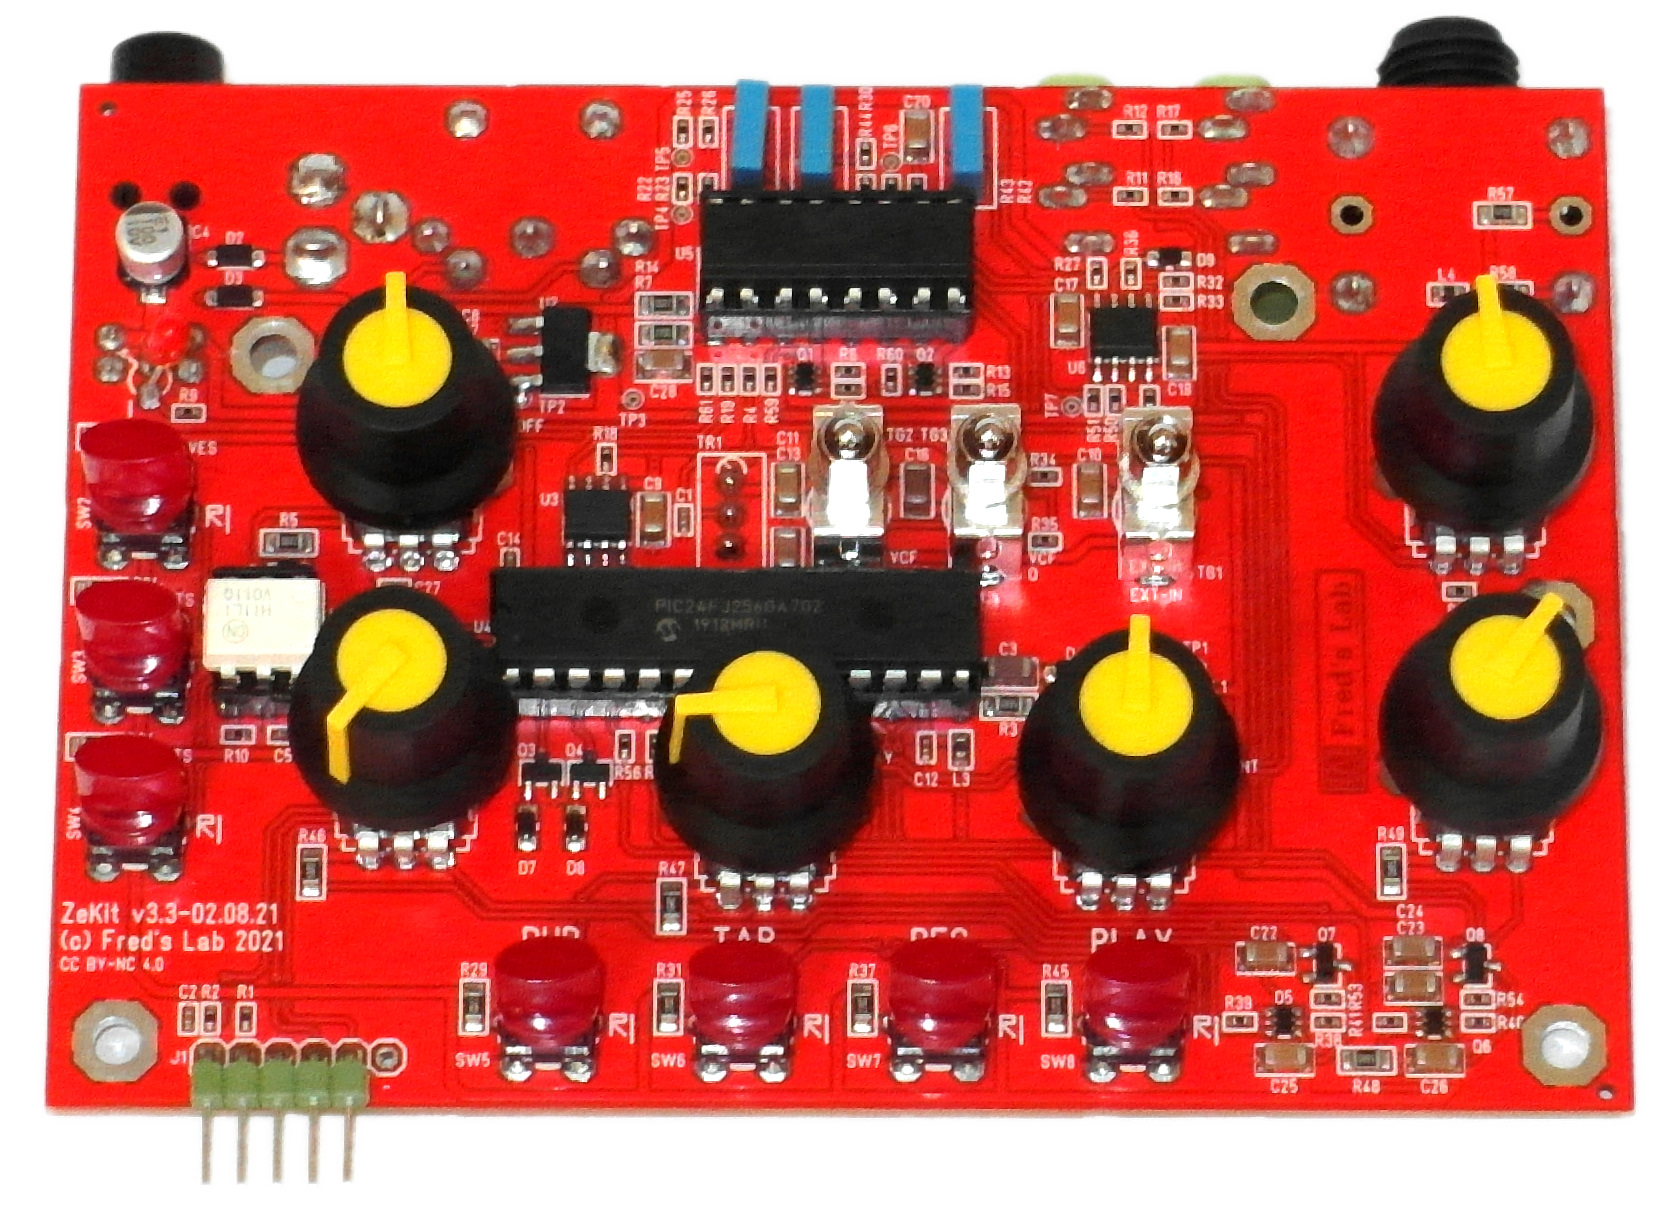
\includegraphics[scale=0.2]{assets/zekit-assembled.jpg}
}
\author{Fred's Lab}

%%% DOCUMENT
\begin{document}

\maketitle

\pagebreak

% ------------------------------------------------------------------------------------------

%%% TABLE OF CONTENTS
\tableofcontents
\pagebreak

% ------------------------------------------------------------------------------------------

\section{Special Thanks}

I would like to thank the following persons for their contributions:

\begin{itemize}
    \item Design consulting: René Schmitz, Oliver Rockstedt
    \item Panel graphics: Serge "erewhon" Beauchamp
    \item Instruction guide: Oliver Rockstedt
    \item Beta-testing: Benoit Ruelle, William Zegal, Mathieu Meslin
\end{itemize}

% ------------------------------------------------------------------------------------------

%%% INTRODUCTION
\section{Introduction}

\textbf{Welcome to the ZeKit assembly guide!}

The \textbf{ZeKit} is a fully functional 4-voice paraphonic synth kit with \textbf{digital oscillators} and \textbf{an analog filter and amplifier.}
It also features \textbf{two analog envelopes} as well as \textbf{a simple pattern sequencer}.
The instrument can be controlled via \textbf{MIDI,} handles \textbf{external clocks} and has \textbf{an audio input.}

Hopefully, \emph{you'll learn a lot} while building this kit and you'll end up with \textbf{an inexpensive and fun instrument} that will quickly integrate your studio setup.

\subsection{Required skills}

\begin{itemize}
    \item \textbf{Basic knowledge of analog synthesis}
    \item Some soldering experience with through-hole components
    \item Some knowledge on how to read a placement diagram
\end{itemize}

\subsection{Required tools}

In order to fully assemble the kit, you'll need the following tools:

\begin{itemize}
    \item A soldering iron with a 3mm flat tip
    \item 1mm solder wire
    \item A wire cutter
    \item A flat head screwdriver
\end{itemize}

\subsection{Required accessories}

\begin{itemize}
    \item A power supply, DC 5 to 9V, 0.5A with a 2.1mm x 5.5mm \\
    center positive barrel connector  (*)
    \item A 6.35mm jack audio cable
    \item Optional / computer, sequencer or MIDI controller
    \item Optional / MIDI cable
\end{itemize}

\vspace{0.25cm}
(*) A compatible power adapter can be purchased from \textbf{Fred's Lab},
but we recommend you \textbf{to reuse} any adapter you already own.

% ------------------------------------------------------------------------------------------
\pagebreak
\section{Box Content}

In addition to \textbf{the pre-assembled PCB,} the \textbf{ZeKit} package contains the following:
\vspace{-0.25cm}

\begin{figure}[!ht]
    \begin{center}
        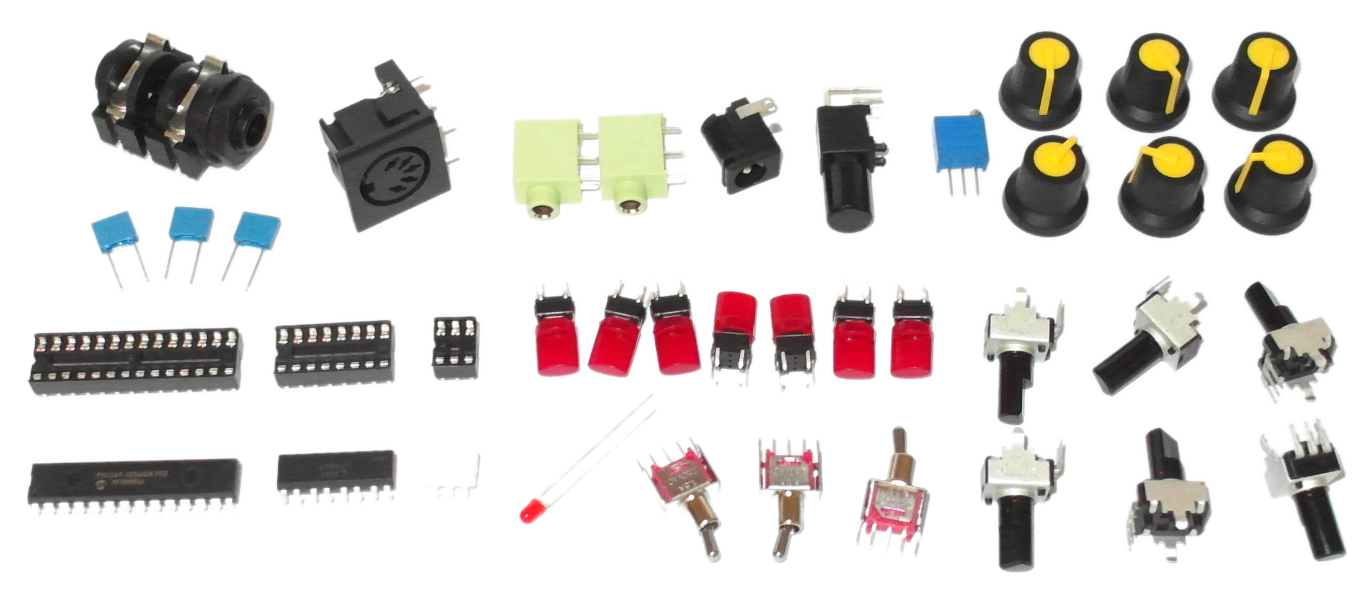
\includegraphics[scale=0.32]{assets/zekit-content.jpg}
        \caption{Components included in the kit}
    \end{center}
\end{figure}

\vspace{0.25cm}

\begin{center}
    \begin{tabular}{|c|l|l|}
        \hline
        \textbf{Amount} & \textbf{Description} & \textbf{Value}  \\
        \hline
        1               & Pre-assembled PCB    &                 \\
        1               & TRS jack socket      & 6.35mm TRS      \\
        1               & DIN5 socket          &                 \\
        2               & TRS jacks socket     & 3.5mm TRS       \\
        1               & Power jack socket    &                 \\
        1               & Power switch         &                 \\
        1               & Trim potentiometer   & 10k Ohm         \\
        6               & Potentiometer knobs  &                 \\
        3               & Film capacitors      & 47nF / 63v      \\
        1               & DIL28 IC socket      &                 \\
        1               & DIL16 IC socket      &                 \\
        1               & DIL6 IC socket       &                 \\
        7               & Tactile switches     &                 \\
        2               & Potentiometers       & 10k Ohm         \\
        4               & Potentiometers       & 100k Ohm        \\
        1               & Microcontroller IC   & PIC24FJ256GA702 \\
        1               & Optocoupler IC       & LTV-847         \\
        1               & Optocoupler IC       & H11L1           \\
        1               & LED                  & 3mm red color   \\
        3               & Toggle switches      &                 \\
        \hline
    \end{tabular}
\end{center}

\vspace{0.5cm}
Before firing up your soldering iron, \textbf{make sure your kit is complete} and take the time \textbf{to get to know} the different components.

\pagebreak
\subsection{Pre-assembled PCB}

The \textbf{ZeKit} makes use of \textbf{SMD} (Surface Mounted Devices) and \textbf{THT} (Through Hole Technology) components. SMD components allow the design to \textbf{remain compact and simple to manufacture} and more cost effective.

\begin{figure}[!ht]
    \begin{center}
        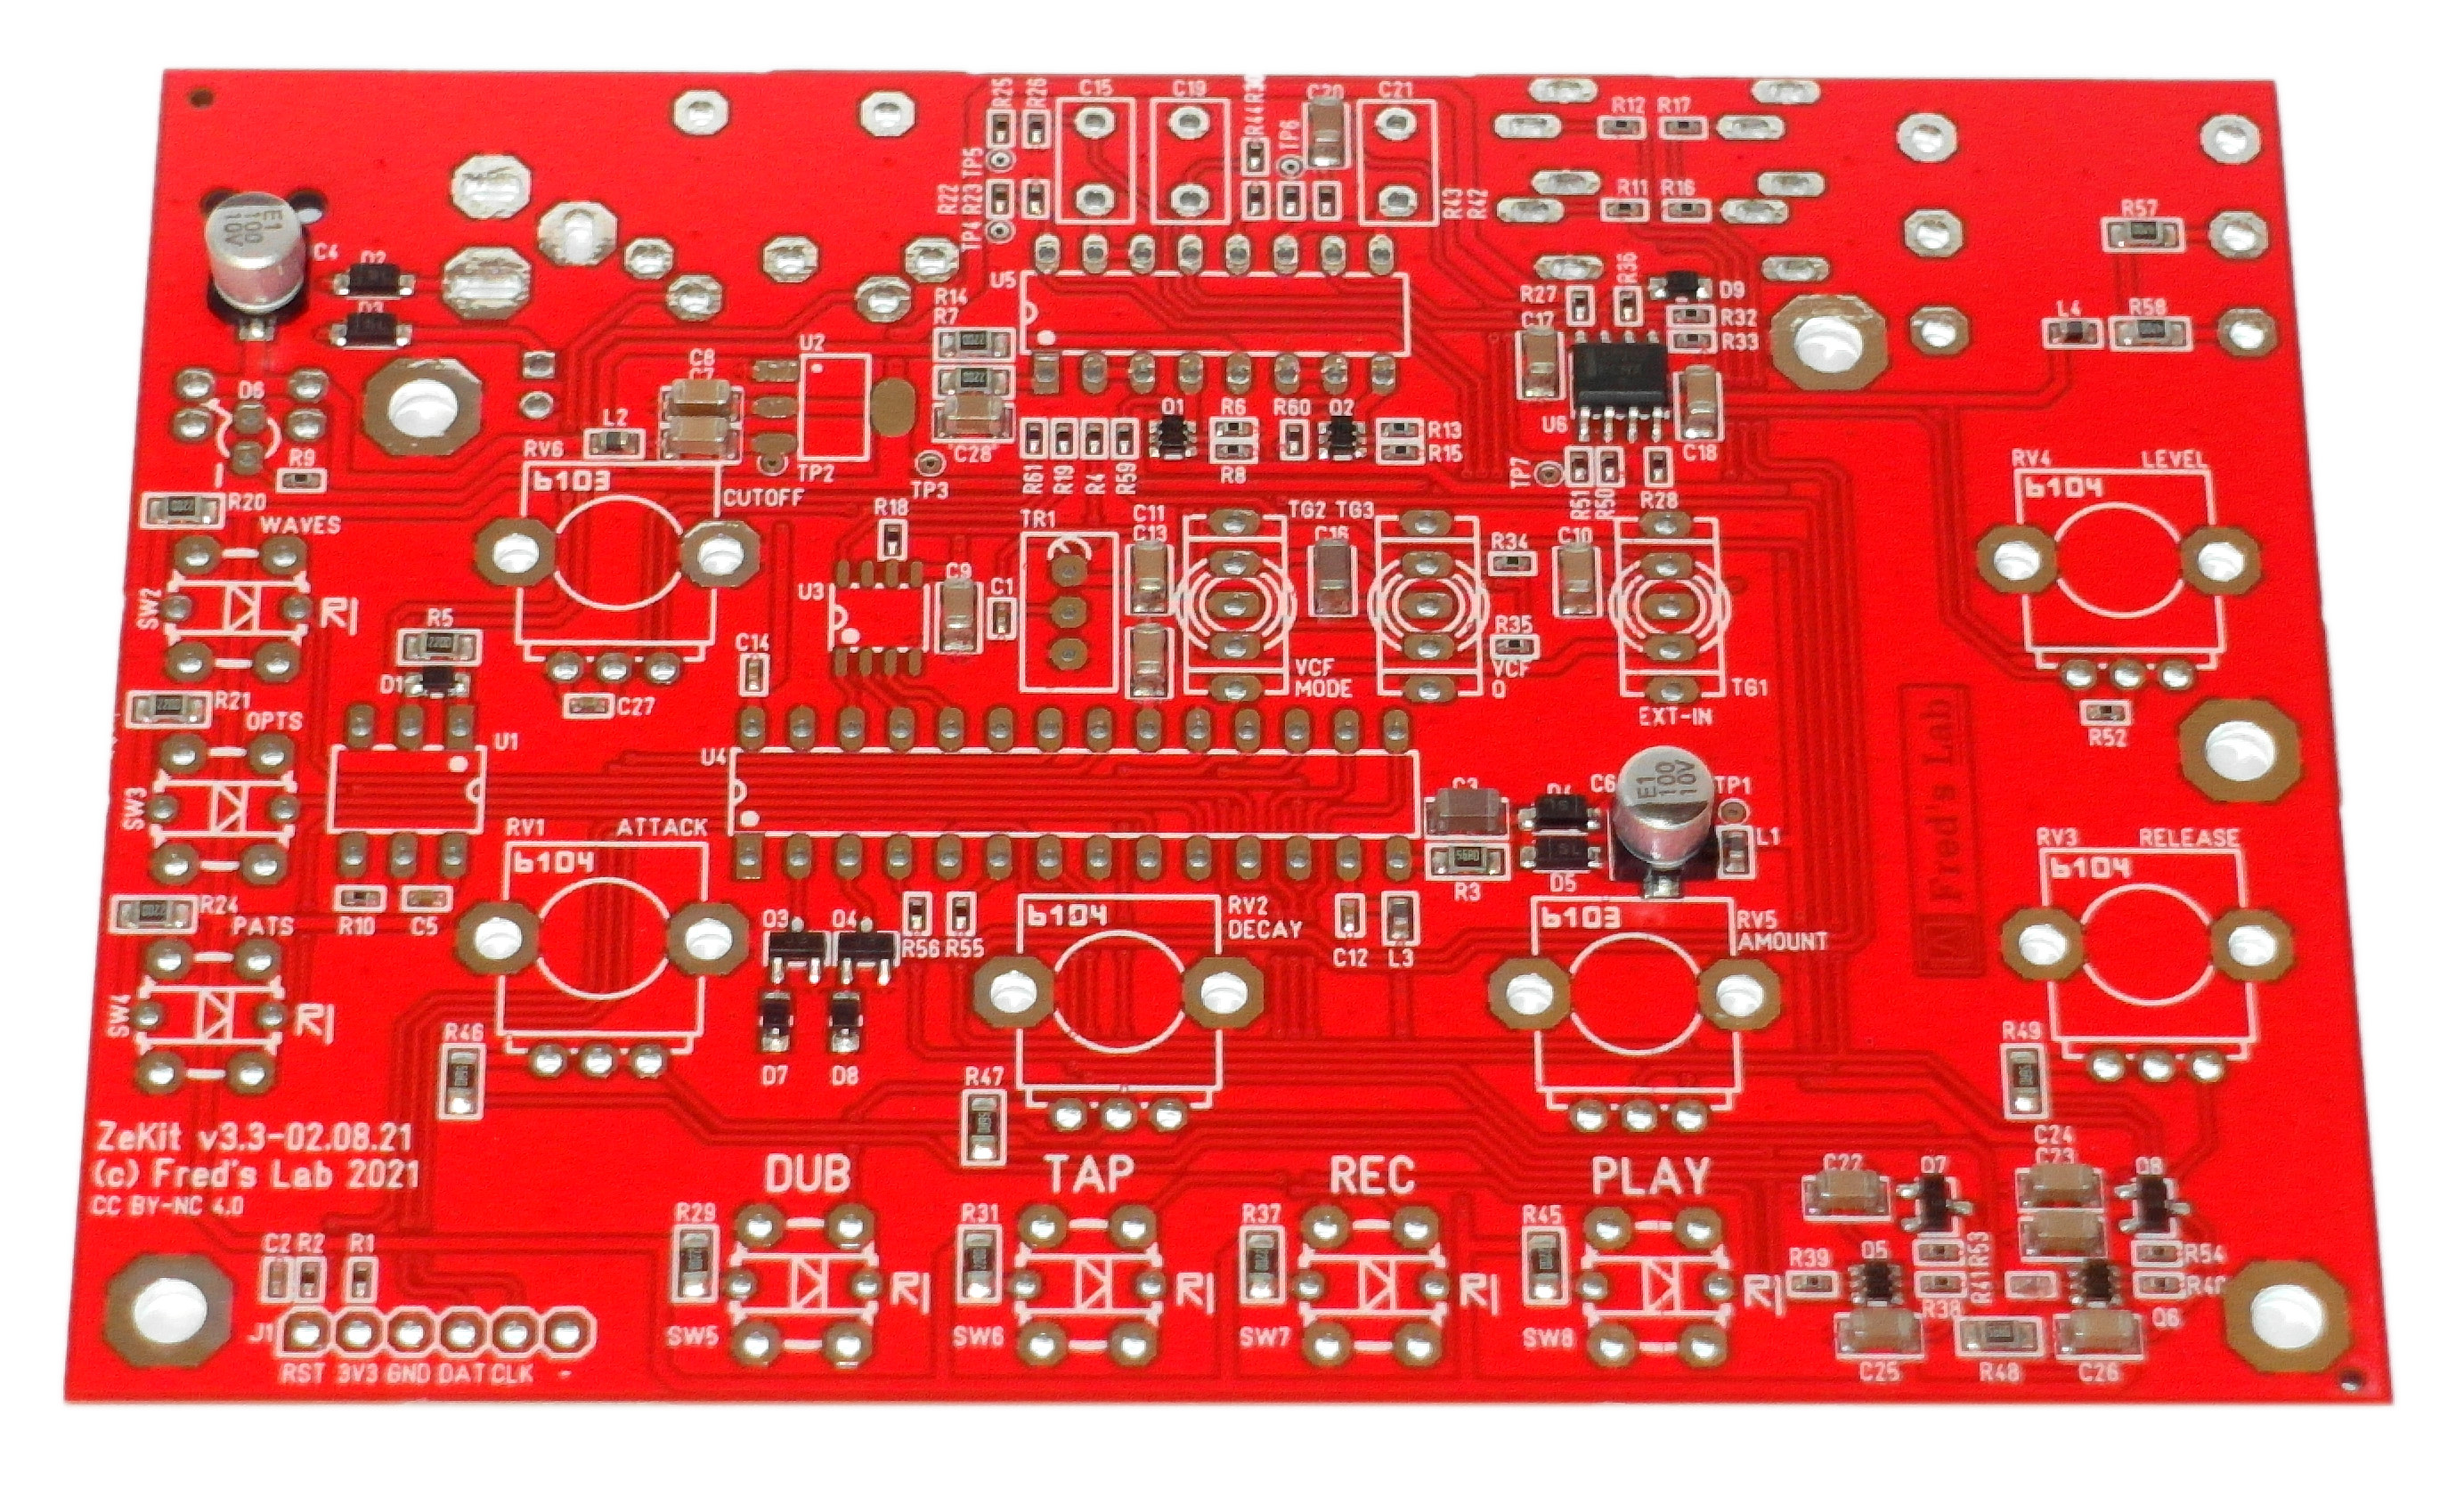
\includegraphics[scale=0.10]{assets/zekit-unassembled.jpg}
        \caption{Pre-assembled ZeKit PCB}
    \end{center}
\end{figure}

All \textbf{SMD components} come already assembled on the \textbf{PCB} (Printed Circuit Board). \\
The \textbf{THT components} are left to be hand soldered, \textbf{and this is your mission!}

\subsection{Learn the Components}

\subsubsection{Power LED}

\begin{figure}[!ht]
    \begin{center}
        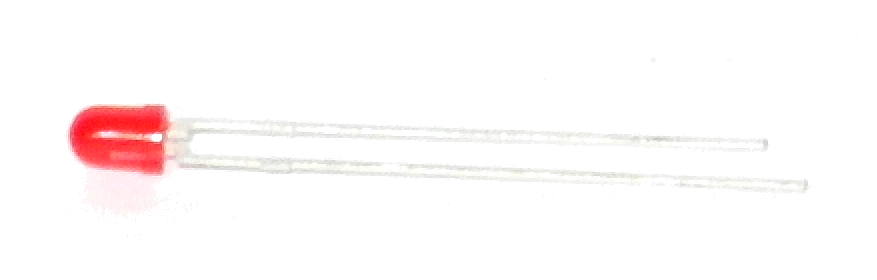
\includegraphics[scale=0.15]{assets/zekit-led.jpg}
        \caption{3mm red LED}
    \end{center}
\end{figure}

The \textbf{LED} (Light Emitting Diode) is an indicator that lights up when a current is running through it.
Here, it shows when the instrument is powered on.

\subsubsection{Tactile Switches}

\begin{figure}[!ht]
    \begin{center}
        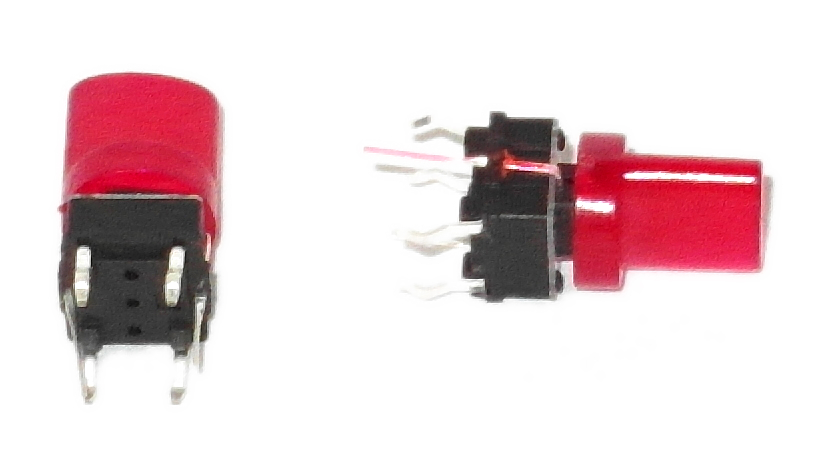
\includegraphics[scale=0.20]{assets/zekit-tacts.jpg}
        \caption{Tactile switches}
    \end{center}
\end{figure}

The \textbf{tactile switches} are \textbf{momentary switches} used as interface buttons.

Their contact is normally open and gets closed when the switch is pressed. These switches have \textbf{an LED built-in} that illuminates the cap to show some status information.

They are connected to the microcontroller directly and are used to select the oscillator waveform, choose the sequencer pattern and toggle various options.

\subsubsection{Toggle Switches}

\begin{figure}[!ht]
    \begin{center}
        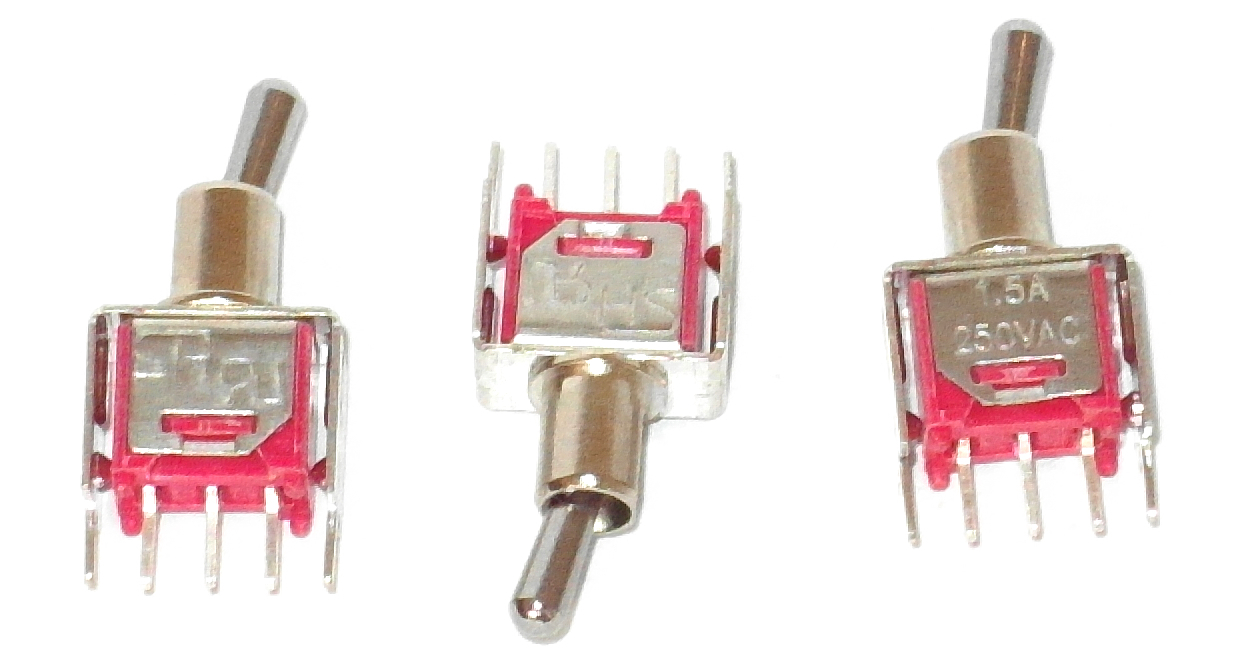
\includegraphics[scale=0.16]{assets/zekit-toggles.jpg}
        \caption{SPDT toggle switches}
    \end{center}
\end{figure}

In contrast to the tactile switches, the \textbf{toggle switches} have \textbf{two stable positions.} They are also called \textbf{SPDT} (single pole, dual throw) switches.
Depending on the lever position, one contact is closed while the other is open and vice versa.

In the \textbf{ZeKit}, these switches select the filter mode (low-pass or band-pass), the filter resonance amount (low or high) and the routing of the external audio input.

\subsubsection{Potentiometers}

\begin{figure}[!ht]
    \begin{center}
        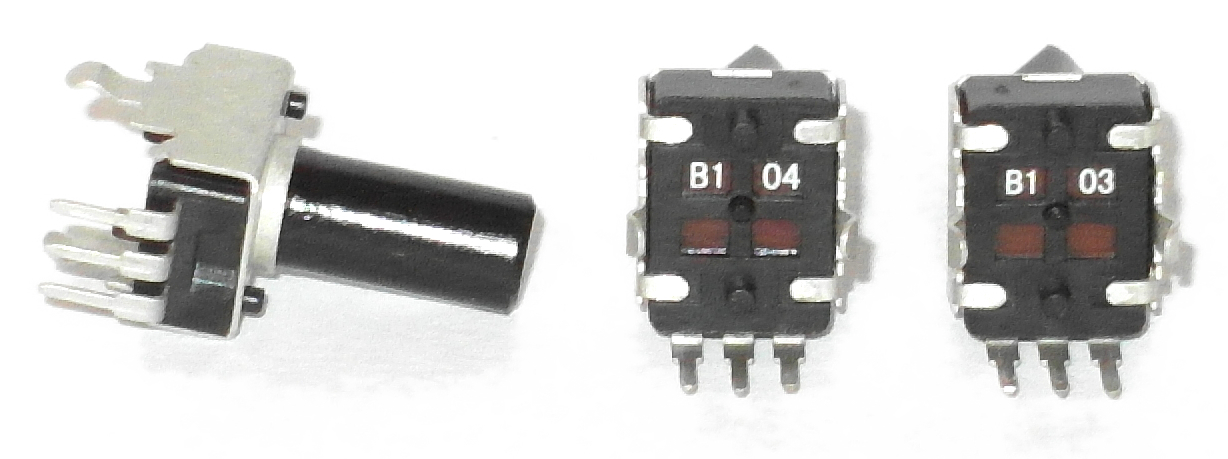
\includegraphics[scale=0.25]{assets/zekit-pots.jpg}
        \caption{Linear mono potentiometers}
    \end{center}
\end{figure}

The \textbf{potentiometers} (or "pots") are \textbf{variable resistors} meant to control sound parameters in the analog domain. They consist of \textbf{a conductive wiper} that slides over a circular \textbf{resistive track} to form a voltage-divider.

The \textbf{ZeKit} uses potentiometers of two different values: \textbf{10k \& 100k Ohm.}

The pots must not be interchanged or the circuit won't work correctly. \\
They can be easily identified by the label found at their bottom:

$\bullet$ \textbf{B103} = 10k Ohm\\
$\bullet$ \textbf{B104} = 100k Ohm\\

\subsubsection{Trimmer}

\begin{figure}[!ht]
    \begin{center}
        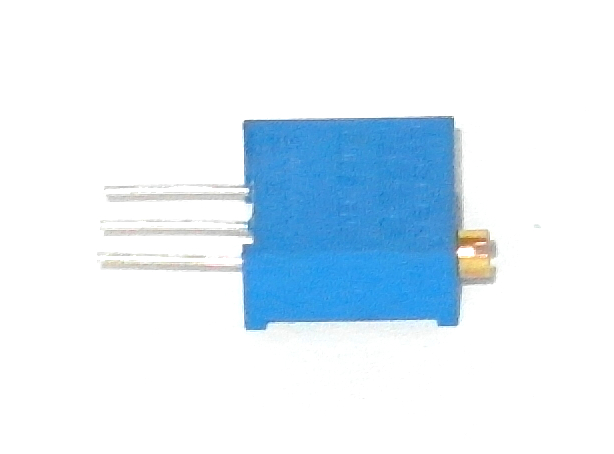
\includegraphics[scale=0.20]{assets/zekit-trimmer.jpg}
        \caption{Multiturn trimmer}
    \end{center}
\end{figure}

\textbf{Trimmers} are specific potentiometers \textbf{intended for calibration} to compensate for the effects of tolerances in other components manufacturing.

These are smaller than regular potentiometers and need to be adjusted with a flathead screwdriver. They offer a \textbf{great setting precision} since their screw can be turned multiple times. They are also called \textbf{multiturn trimmers}.

The \textbf{ZeKit} uses a single trimmer to define the filter \textbf{cutoff frequency} range.

\subsubsection{Power Switch}

\begin{figure}[!ht]
    \begin{center}
        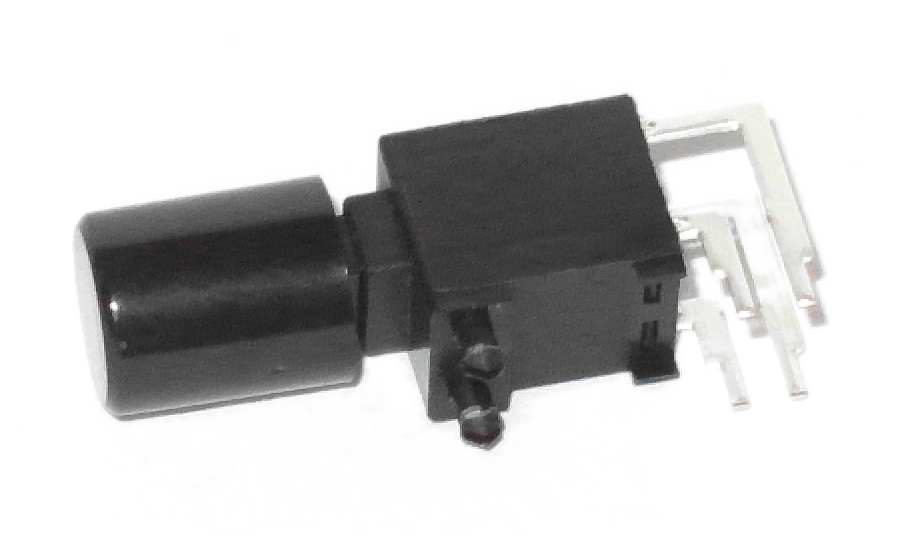
\includegraphics[scale=0.18]{assets/zekit-power.jpg}
        \caption{Power switch}
    \end{center}
\end{figure}

The \textbf{power switch} is a \textbf{latching push button} with a toggle behavior. \\
Pressed once, the contact closes and remains in this state until it is pressed again.

This switch turns the \textbf{ZeKit} power on or off.

\subsubsection{Power Jack Socket}

\begin{figure}[!ht]
    \begin{center}
        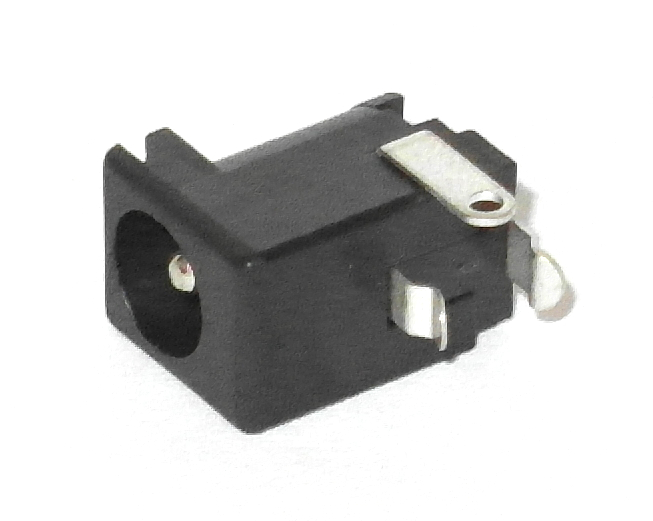
\includegraphics[scale=0.15]{assets/zekit-dcjack.jpg}
        \caption{Power jack socket}
    \end{center}
\end{figure}

The \textbf{power jack} is a standard 2.1mm barrel or coaxial connector that has a widespread use with low voltage power supplies.

The \textbf{ZeKit} can be powered from any DC (direct current) adapter with a voltage ranging from 5V to 9V. The center connection must be positive.

\subsubsection{DIN5 Socket}

\begin{figure}[!ht]
    \begin{center}
        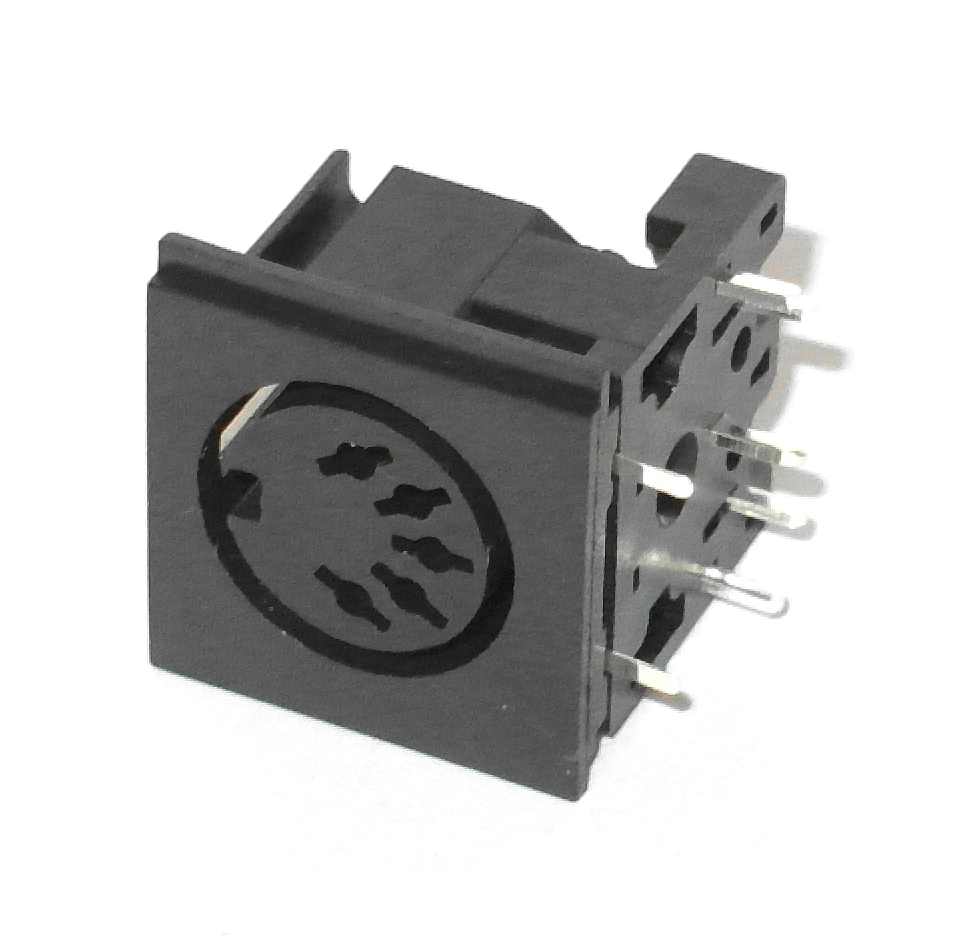
\includegraphics[scale=0.20]{assets/zekit-din.jpg}
        \caption{DIN5 socket}
    \end{center}
\end{figure}

The \textbf{DIN5 socket} is a 5-pin connector used for \textbf{MIDI input}. \textbf{MIDI} stands for \textbf{Music Instrument Digital Interface} and allows the \textbf{ZeKit} to play notes and be synchronized rhythmically with other compatible gear, like controllers or sequencers.

\subsubsection{6.35mm TS Jack Socket}

\begin{figure}[!ht]
    \begin{center}
        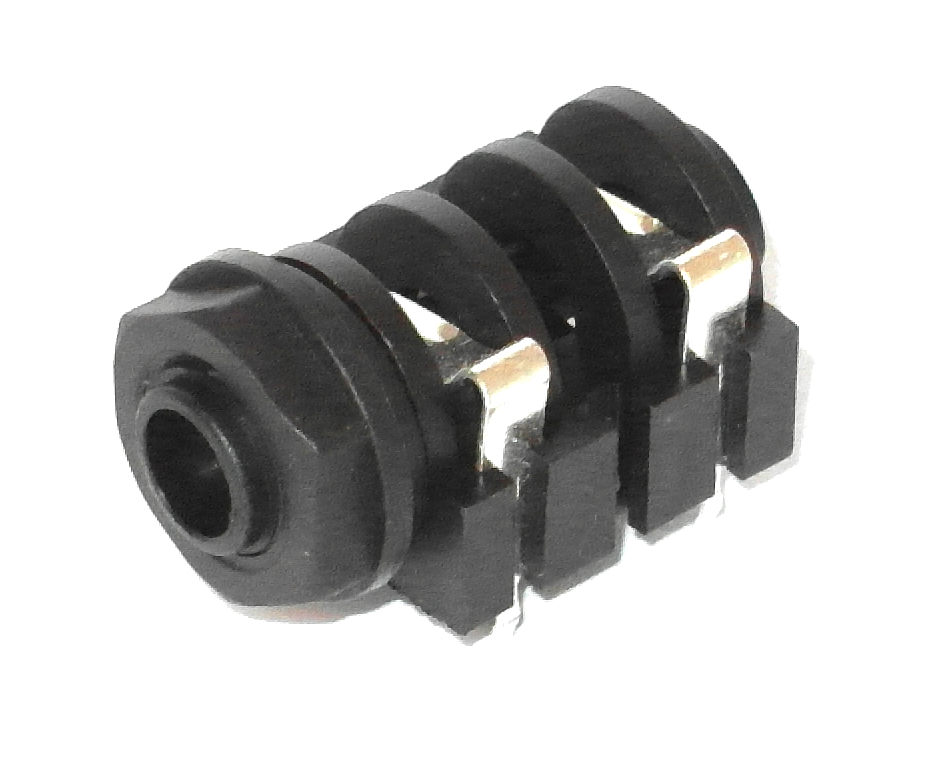
\includegraphics[scale=0.20]{assets/zekit-jack.jpg}
        \caption{6.35mm Jack Socket}
    \end{center}
\end{figure}

The \textbf{TS jack} stands for "tip and sleeve". This connector is common in \textbf{audio systems} to transmit the sound. The sleeve connection is always grounded whereas the tip carries the mono or "left" audio signal. An optional "ring" connection will carry the "right" signal.

This connector is used as the \textbf{ZeKit} line and, optionally, headphones output.

\pagebreak
\subsubsection{3.5mm TRS Jack Sockets}

\begin{figure}[!ht]
    \begin{center}
        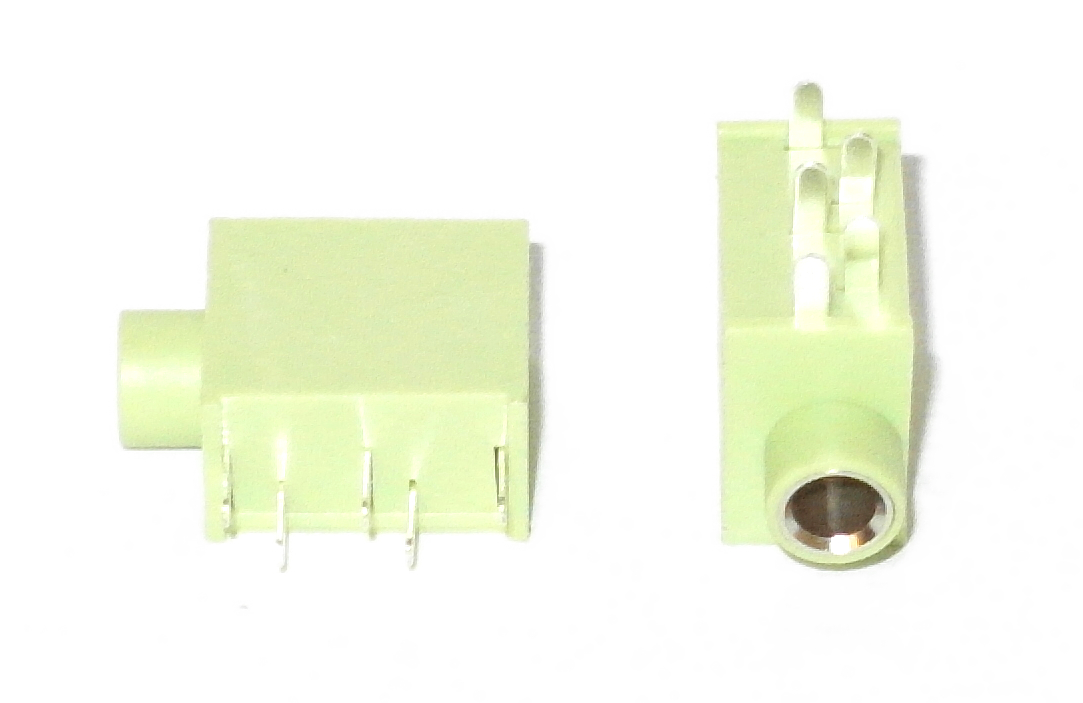
\includegraphics[scale=0.15]{assets/zekit-minijack.jpg}
        \caption{3.5mm Jack Sockets}
    \end{center}
\end{figure}

These sockets are smaller and stereo versions of the 6.35mm ones. In the \textbf{ZeKit}, they are used for the \textbf{external audio} and the \textbf{clock or "sync"} inputs.

The \textbf{clock signal} is expected on the jack tip and the sequencer running state (start or stop) on the ring connection. The sleeve connection is grounded.

\subsubsection{Film Capacitors}

\begin{figure}[!ht]
    \begin{center}
        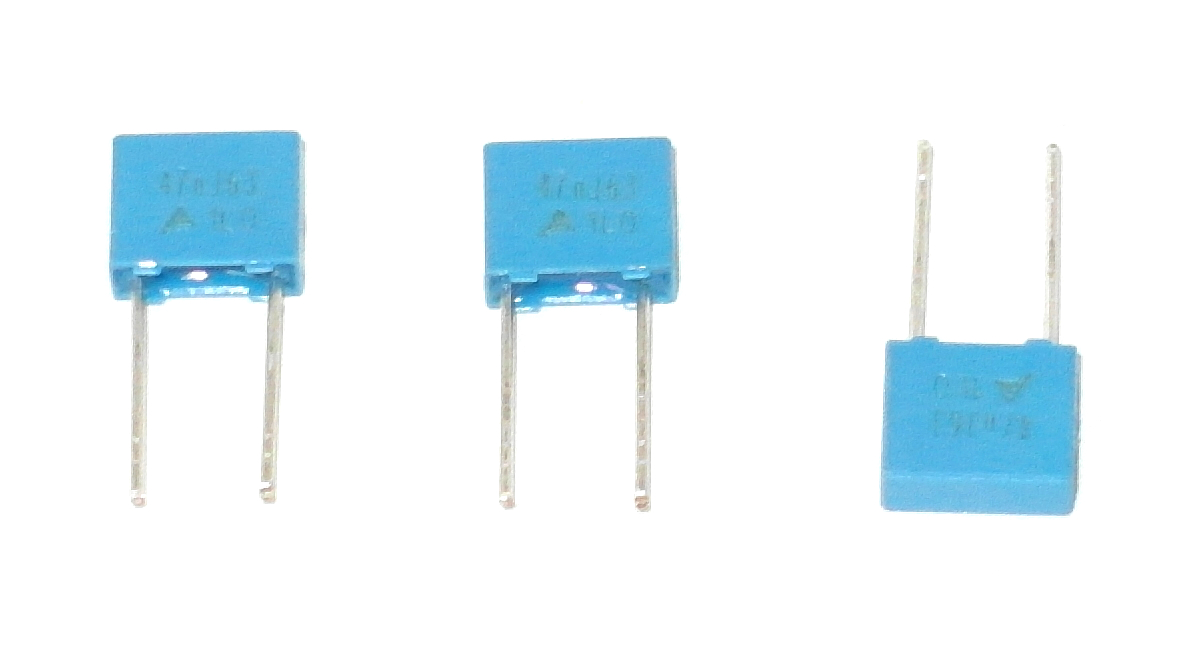
\includegraphics[scale=0.15]{assets/zekit-caps.jpg}
        \caption{47nF Film Capacitors}
    \end{center}
\end{figure}

The \textbf{film capacitors} are capacitors or "caps", they can \textbf{store and release energy.} These types are superior to standard ceramic ones, in terms of \textbf{distortion and noise immunity.}
They also have tighter capacity tolerances.

In the \textbf{ZeKit}, they are used in the voltage controlled filter and amplifier circuits to process the audio signal.

\pagebreak
\subsubsection{PIC Microcontroller IC}

\begin{figure}[!ht]
    \begin{center}
        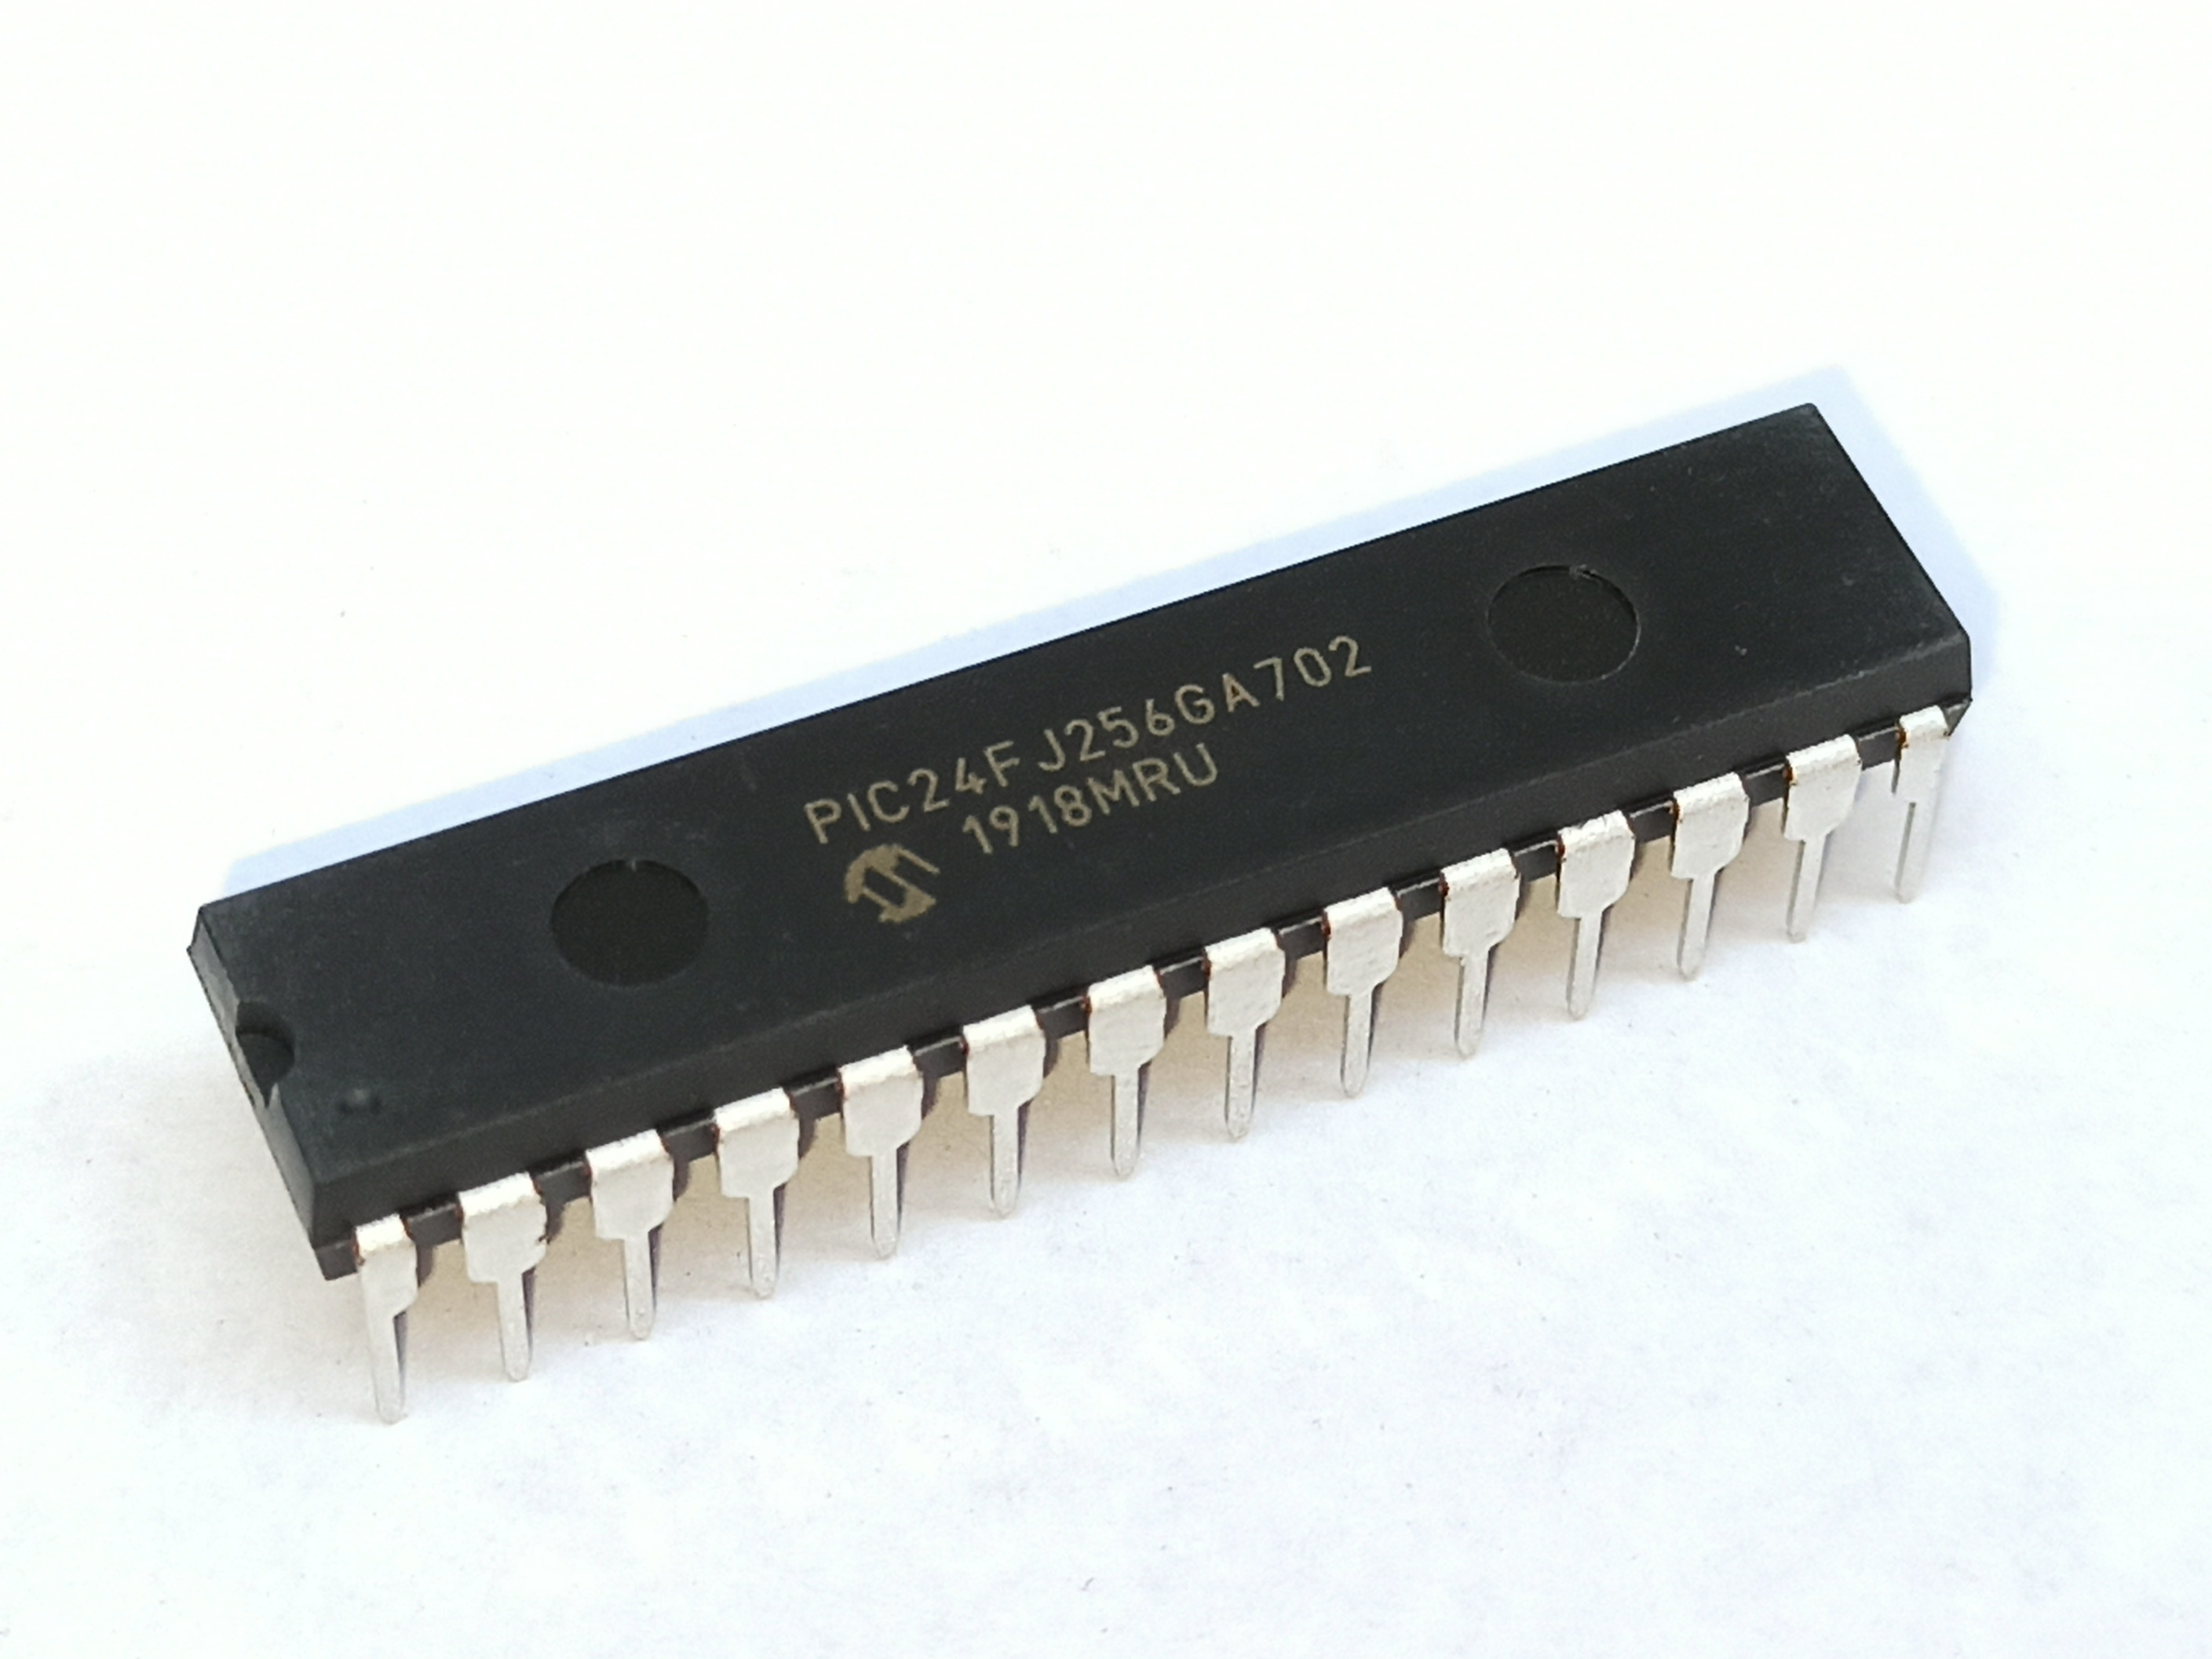
\includegraphics[scale=0.10]{assets/zekit-mcu.jpg}
        \caption{PIC24F 16bit MCU}
    \end{center}
\end{figure}

The \textbf{microcontroller} or "MCU" (Micro-Controller Unit) is an IC (integrated circuit) that contains a \textbf{complete computer.} It features flash memory to store the firmware, RAM to hold data and a processing core with a number of integrated peripherals to communicate with external components.

The \textbf{ZeKit} MCU has a \textbf{16-bit architecture} running at 16Mhz. Its job is to process incoming MIDI messages, handle clock signals, generate the waveforms, run the sequencer, control the envelopes and manage the user interface (buttons and LEDs).

The firmware handling these tasks comes pre-programmed by \textbf{Fred’s Lab,} but it can be modified and replaced by the user, using special tools.

\subsubsection{Optocoupler ICs}

\begin{figure}[!ht]
    \begin{center}
        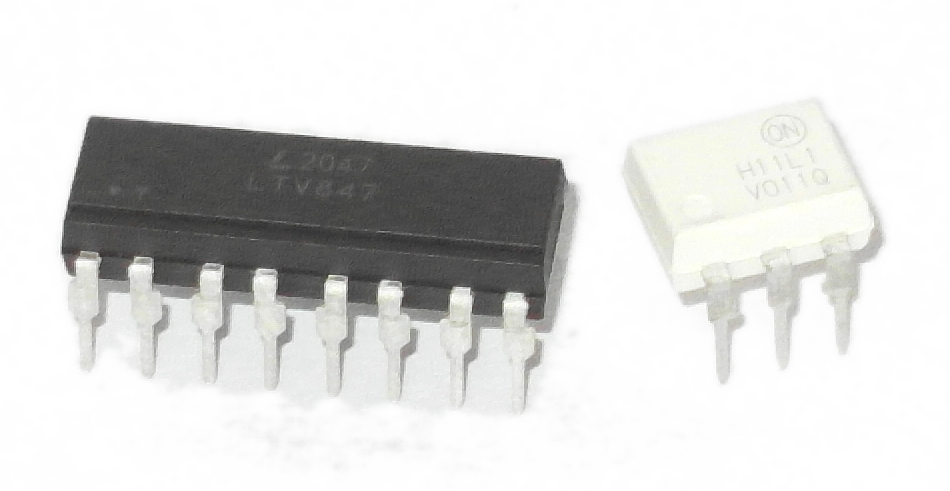
\includegraphics[scale=0.20]{assets/zekit-optocouplers.jpg}
        \caption{Single and quad optocouplers}
    \end{center}
\end{figure}

An \textbf{optocoupler} is a combination of a \textbf{photo transistor} and an \textbf{LED} inside a light sealed package. It is used keep circuits \textbf{electrically isolated} while transferring signals.

The conductance of the photo transistor is related to the brightness of the LED.

The \textbf{ZeKit} uses optocouplers for the \textbf{MIDI input} and as \textbf{current controlled resistors} in the VCF (voltage controlled filter) and VCA (voltage controlled amplifier) sections.

\pagebreak
\subsubsection{DIP Sockets}

\begin{figure}[!ht]
    \begin{center}
        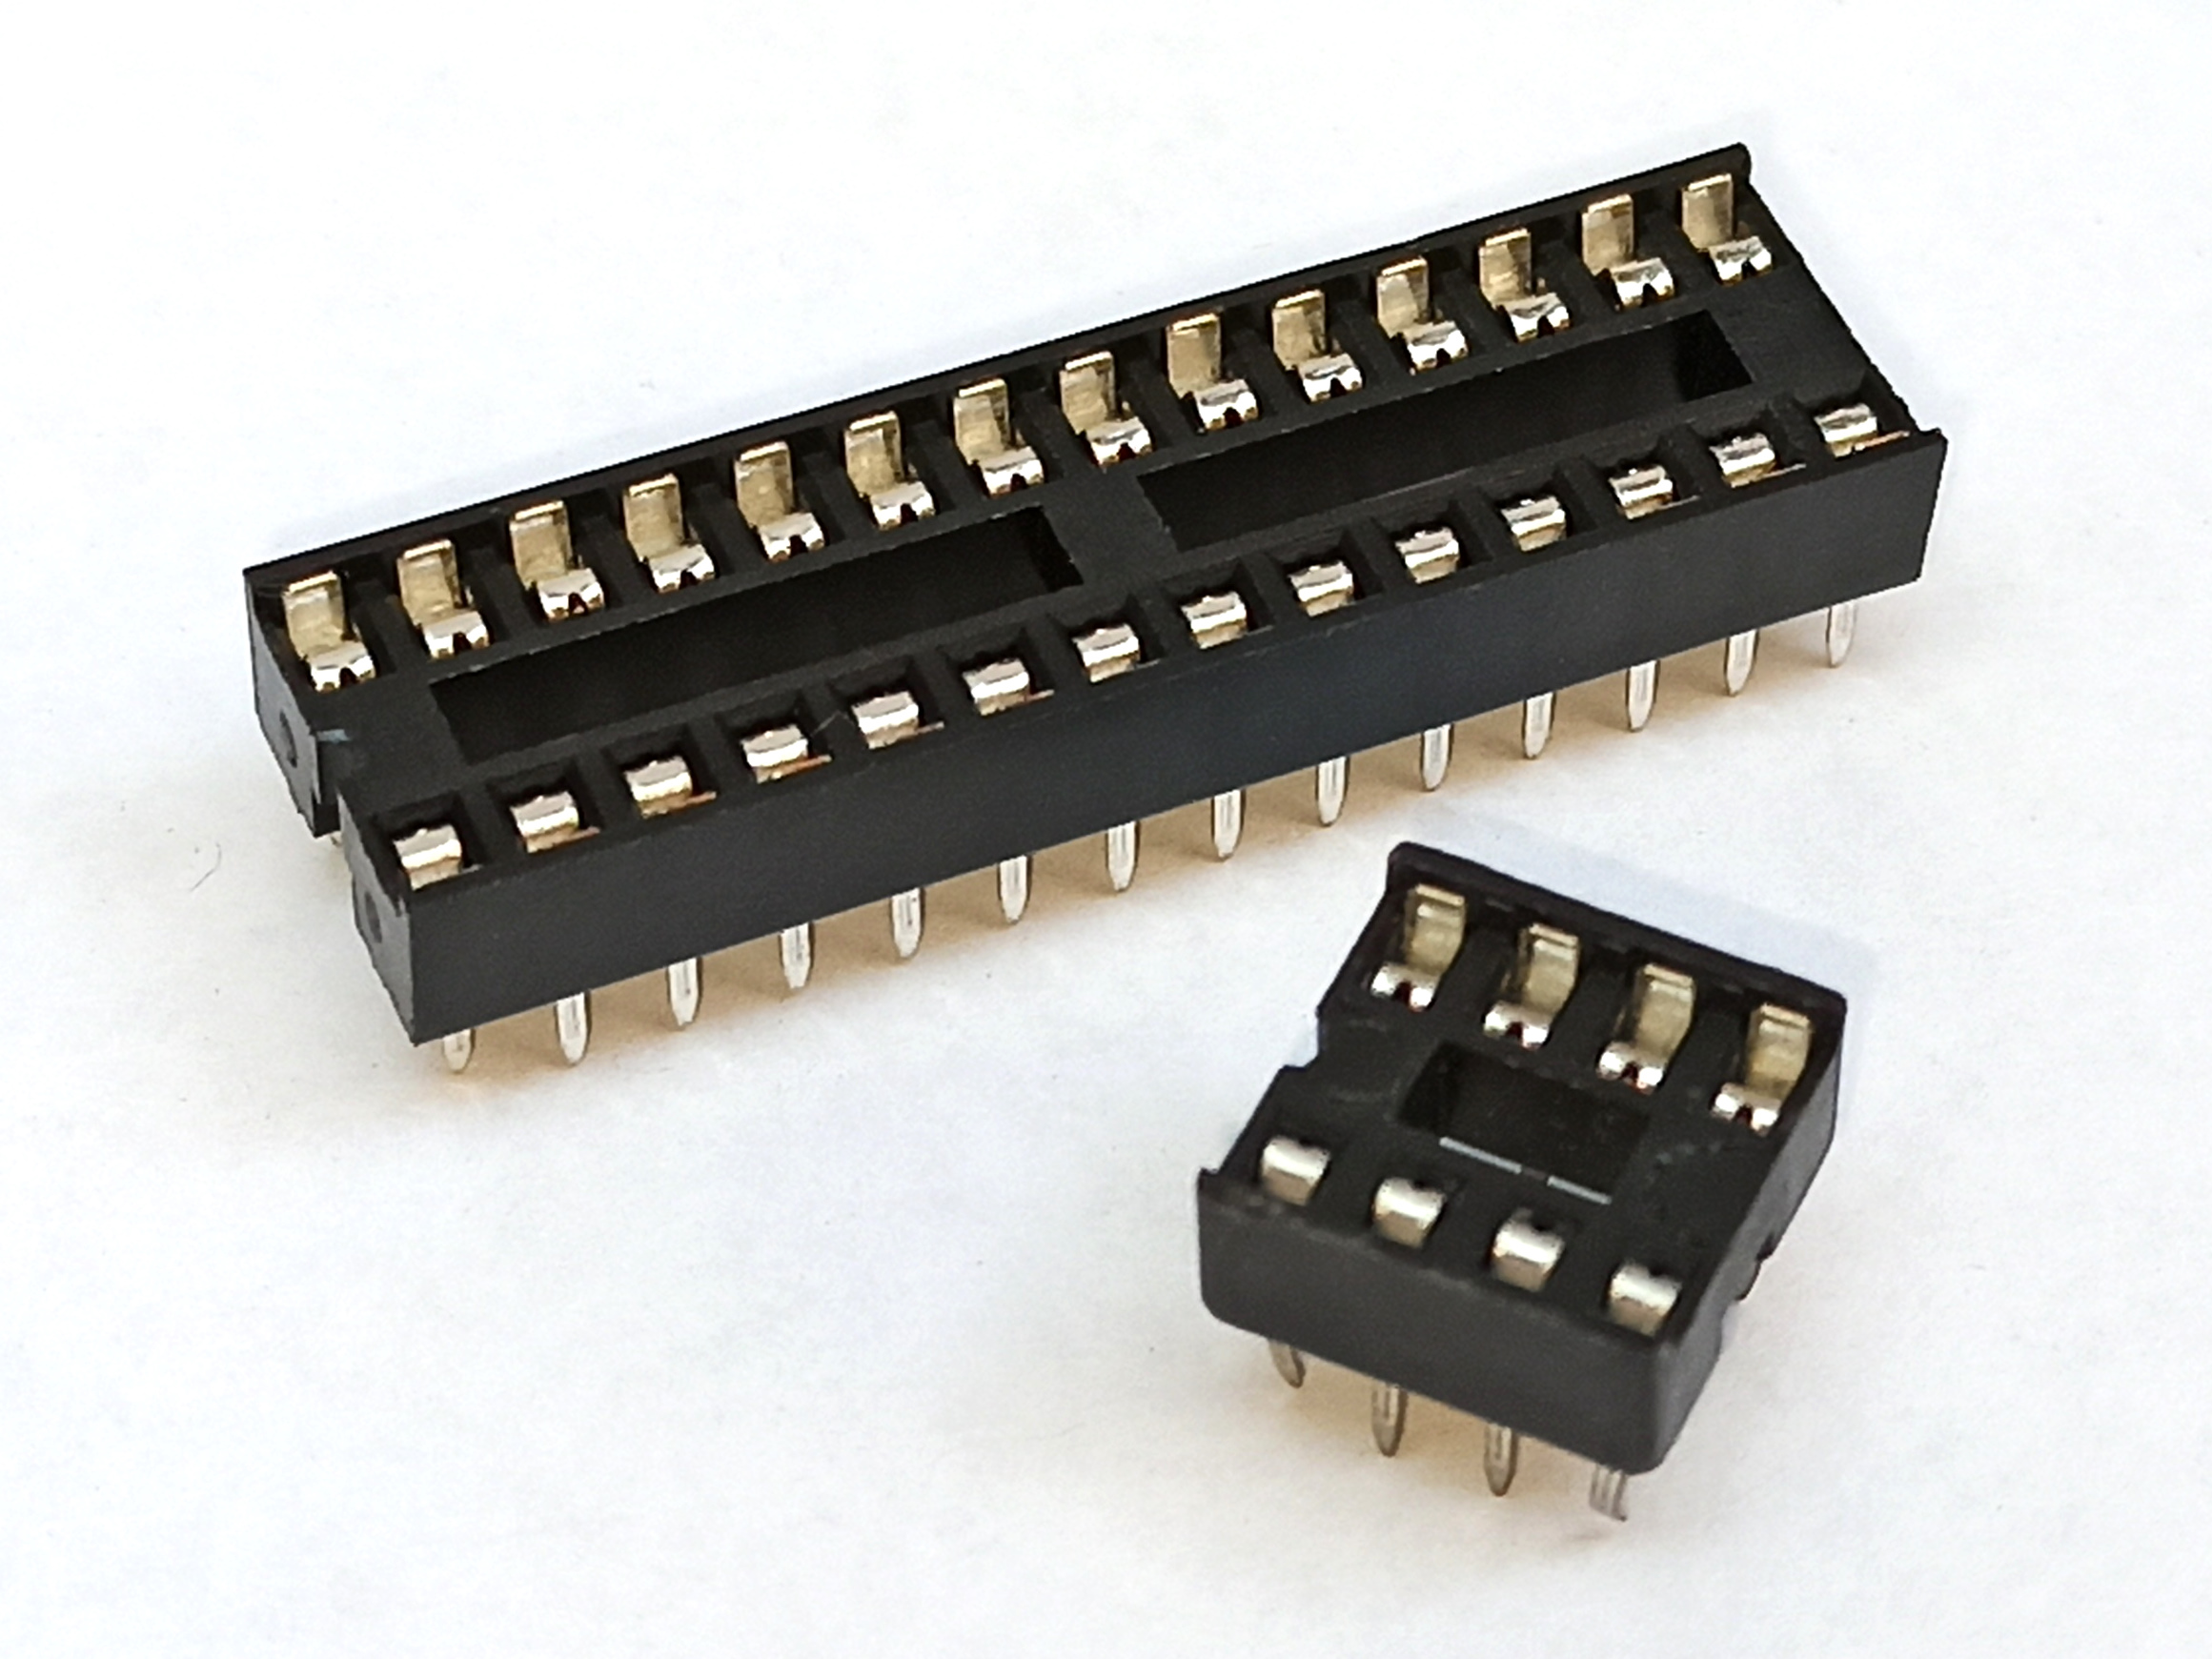
\includegraphics[scale=0.20]{assets/zekit-sockets.jpg}
        \caption{DIP Sockets}
    \end{center}
\end{figure}


Instead of directly soldering the ICs onto the PCB, \textbf{DIP Sockets} (Dual In-line Package) are preferably installed first.

They will \textbf{protect the ICs from soldering heat and keep them exchangeable.} \\
Using sockets, ICs also can't be soldered "the wrong way"... \\
Don't worry, this has happened to the best of us!

\subsubsection{Knobs}

\begin{figure}[!ht]
    \begin{center}
        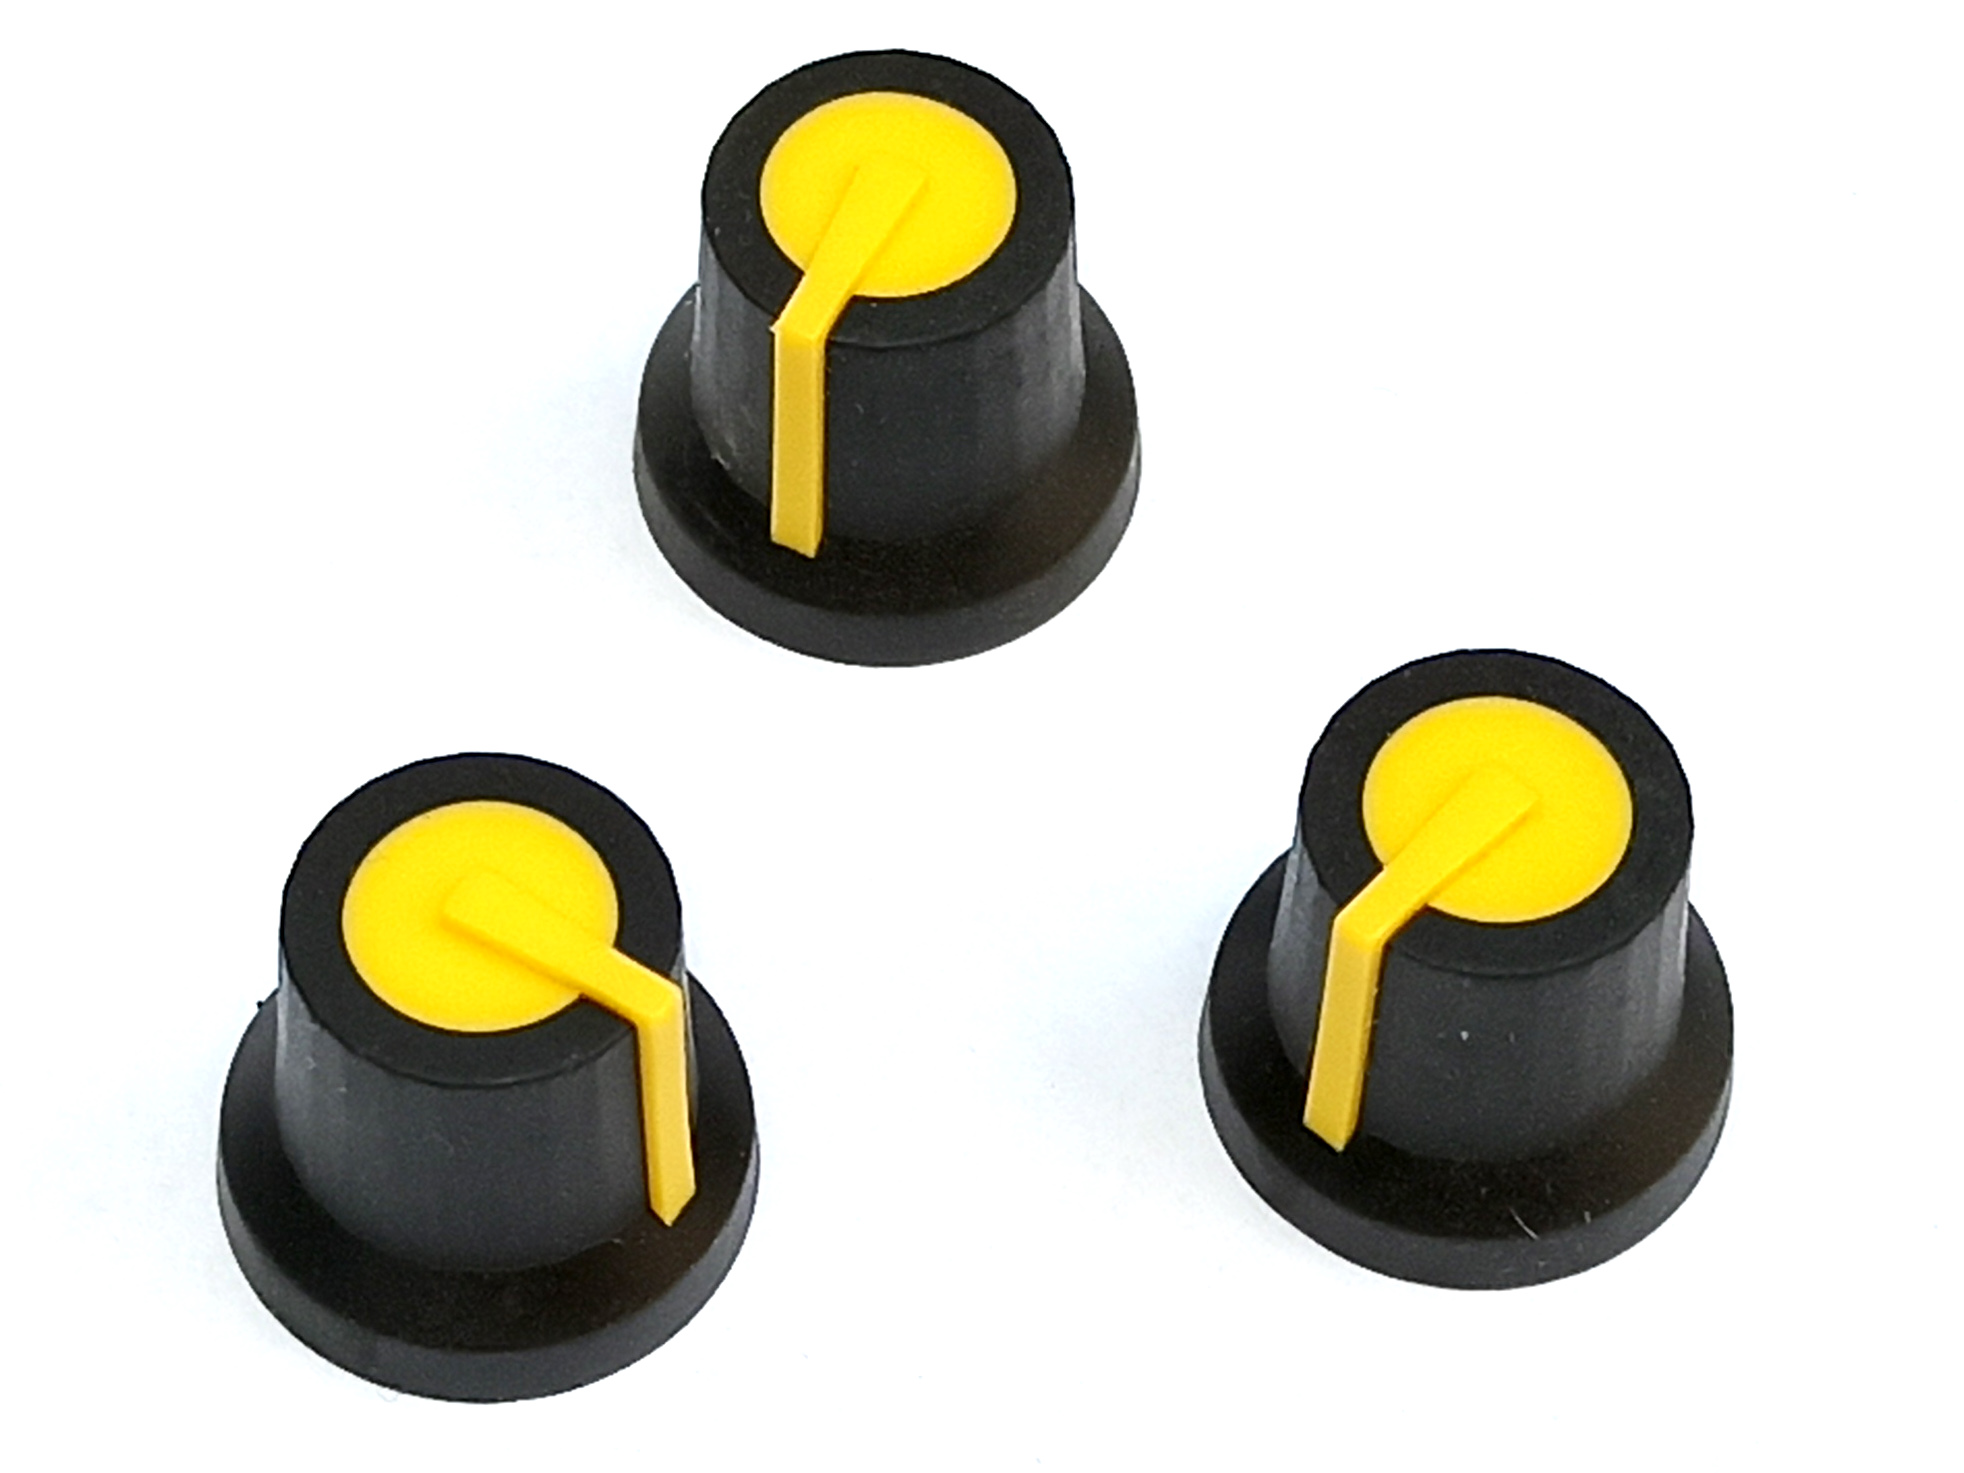
\includegraphics[scale=0.20]{assets/zekit-knobs.jpg}
        \caption{Potentiometer Knobs}
    \end{center}
\end{figure}

\textbf{The knobs} are fitted onto the pots, after the kit is \textbf{fully assembled}, and only then!.

They contribute to the \textbf{final look-and-feel} and allow precise control of the potentiometers and the associated sound settings.

\pagebreak

% ------------------------------------------------------------------------------------------
\section{Assembling the Kit}

\subsection{General Advice}

To maximize your chance of success assembling the \textbf{ZeKit,} work preferably on a \textbf{tidy \& properly lit} surface.
Don't hesitate to \textbf{use magnification} to control your solder joints, reheat with \emph{no-clean flux}, when necessary.
Keep unused parts in their original packaging, so you won't loose them.

Soldering is easier with a \textbf{clean and not oxidized} iron tip. Always \textbf{switch off your iron} when not soldering to extend your tip lifespan!

\subsection{Setting up the soldering gig}

\begin{itemize}
    \item Only work in a well-ventilated room
    \item Use SnCuNiGe (SN100C), SN96.5Ag3Cu0.5 (SAC305) or Sn60Pb40 solder wire
    \item Regularly clean the tip with a wet sponge
    \item Have some duct tape or blu tack at hand
\end{itemize}

\subsection{How to solder like a Pro}

Great solder joints can be achieved \emph{even with basic equipment} and little practice,\\
by following these steps:

\begin{enumerate}
    \item Position (and secure) the component properly
    \item Apply heat to the PCB pad first with the iron tip
    \item Bring in the solder wire until there is enough material
    \item Pull back the solder wire still heating the joint
    \item Pull back the tip from the joint
    \item Let the solder joint cool down naturally - don't blow on it
\end{enumerate}

\pagebreak
\textbf{Illustrated soldering process:}

\begin{center}
    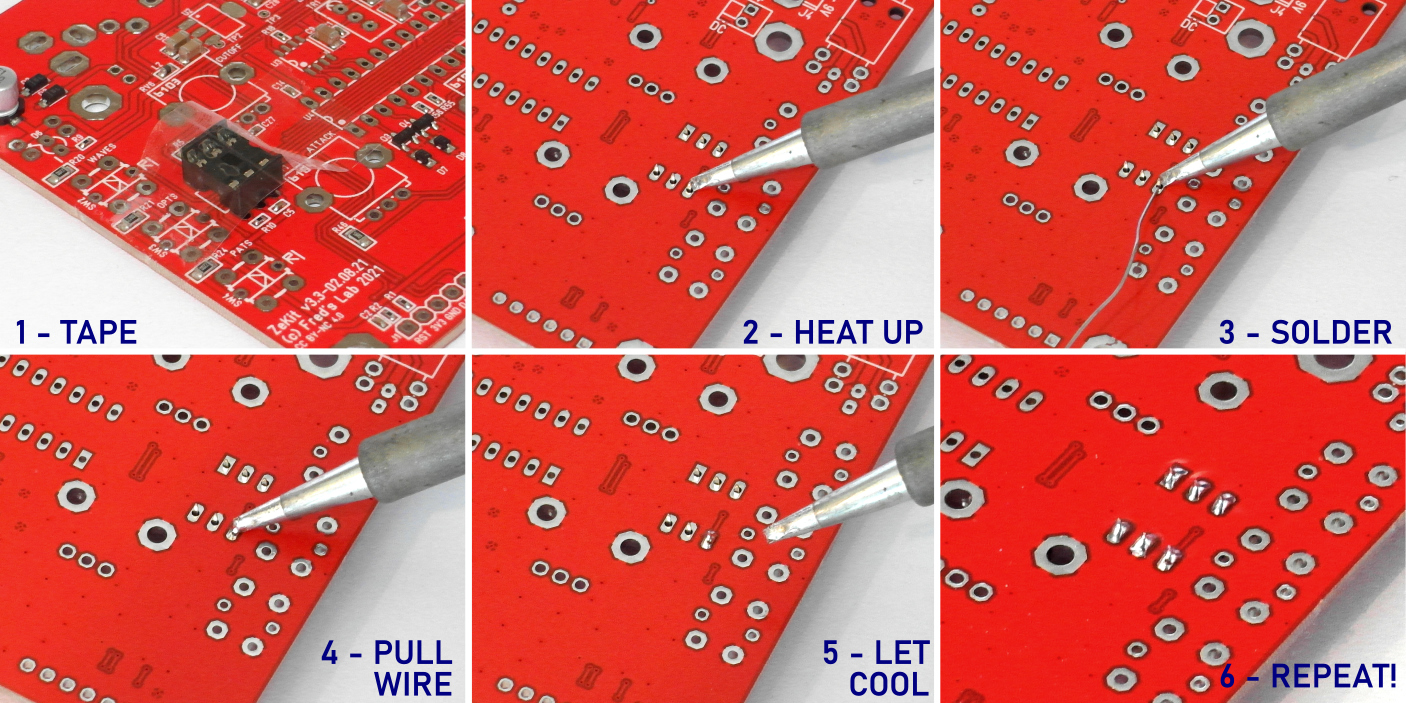
\includegraphics[scale=0.65]{assets/solder-strip.jpg}
\end{center}

\vspace{0.50cm}
\textbf{Additional Tips:}

\begin{itemize}
    \item Tape or tack the components before soldering
    \item Double-check the components orientation
    \item Verify sockets notch match with footprint
    \item Ensure the board is clean before soldering
    \item Optional - use isopropyl alcohol (propan-2-ol) to clean the board
    \item Optional - apply \emph{no-clean flux} on pads and legs
\end{itemize}

\vspace{0.25cm}

\begin{figure}[!ht]
    \begin{center}
        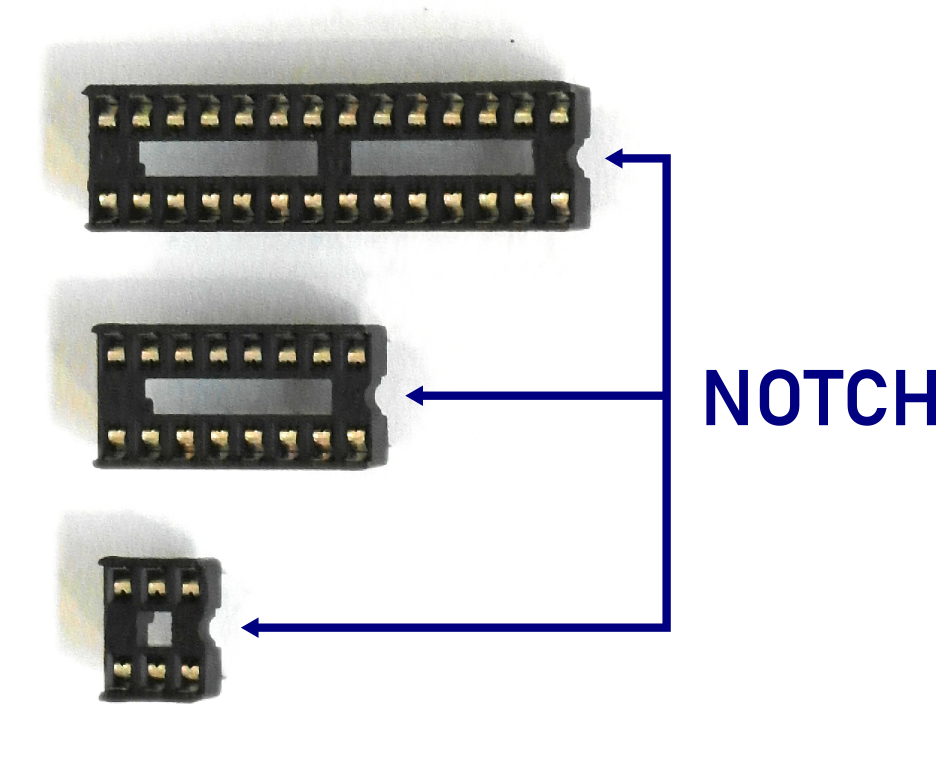
\includegraphics[scale=0.38]{assets/ic-notch.png}
        \caption{IC sockets notch}
    \end{center}
\end{figure}

\pagebreak
\subsection{Soldering the Components}
\Large
Let's heat-up that iron!
\normalsize

The electronic parts are best soldered in \textbf{a specific order} that is determined by their placement and their size.

You can \textbf{tape or tack the parts} to prevent them from falling off when turning over the PCB for soldering.
All potentiometers, switches and connectors \textbf{must be soldered as straight as possible.}

\begin{figure}[!ht]
    \begin{center}
        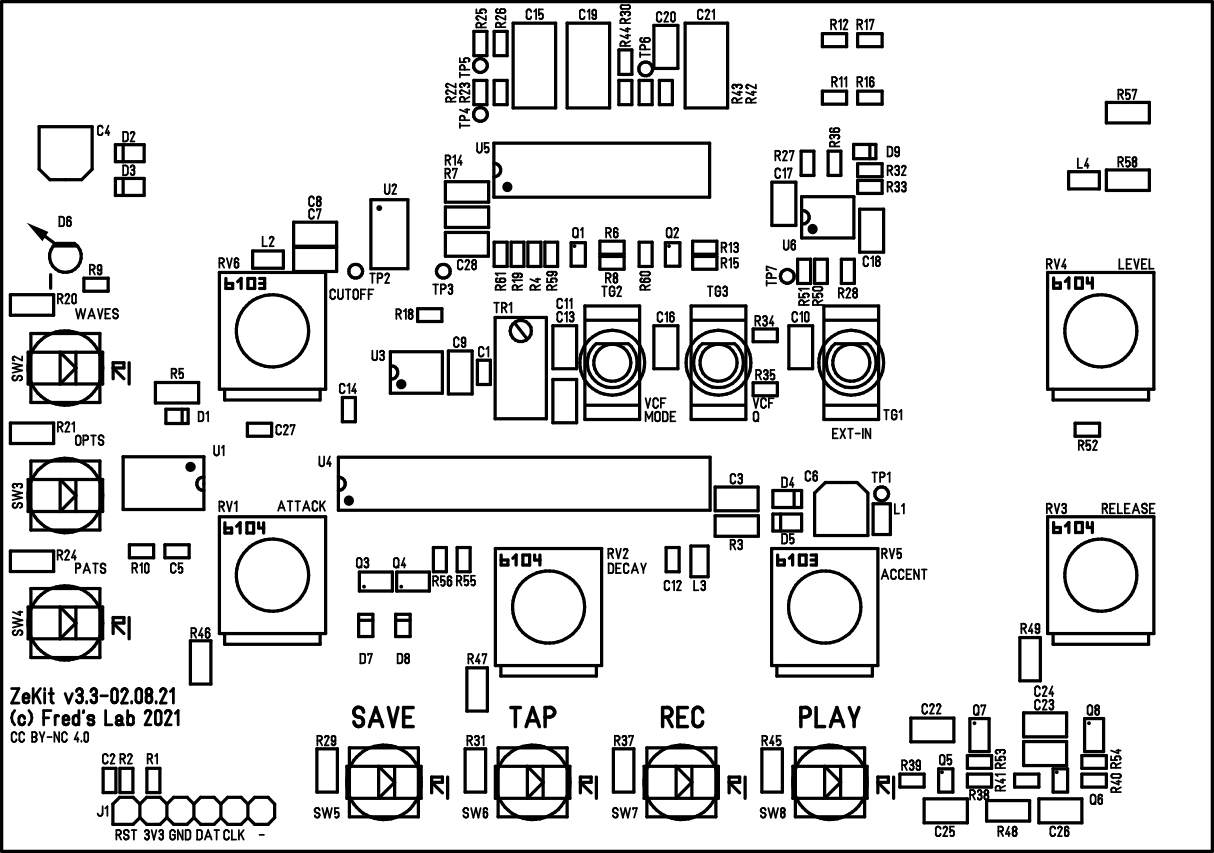
\includegraphics[scale=0.70]{assets/pcb-top.png}
        \caption{Top placement diagram}
    \end{center}
\end{figure}

\vspace{0.5cm}
\textbf{IMPORTANT}

\begin{tcolorbox}
    \textcolor{red}{
        Some parts have a polarity and \textbf{must be soldered in the right orientation.} These components may fit in more than one way but using a wrong orientation will result in erroneous operation or can destroy them.
    }
\end{tcolorbox}

\vspace{0.25cm}

\begin{tcolorbox}
    \textcolor{red}{
        All connectors and the power switch are located \textbf{on the bottom side} of the PCB and must be soldered \textbf{from the top.}
    }
\end{tcolorbox}

\vspace{0.25cm}
\begin{tcolorbox}
    \textcolor{red}{
        \textbf{De-soldering a part} which has been incorrectly mounted \textbf{is tedious} and requires good soldering experience and specific tools. To avoid this, better check the part placement twice \textbf{before soldering.}
    }
\end{tcolorbox}

\pagebreak
\subsubsection{Step 1: IC Sockets}

\begin{figure}[!ht]
    \begin{center}
        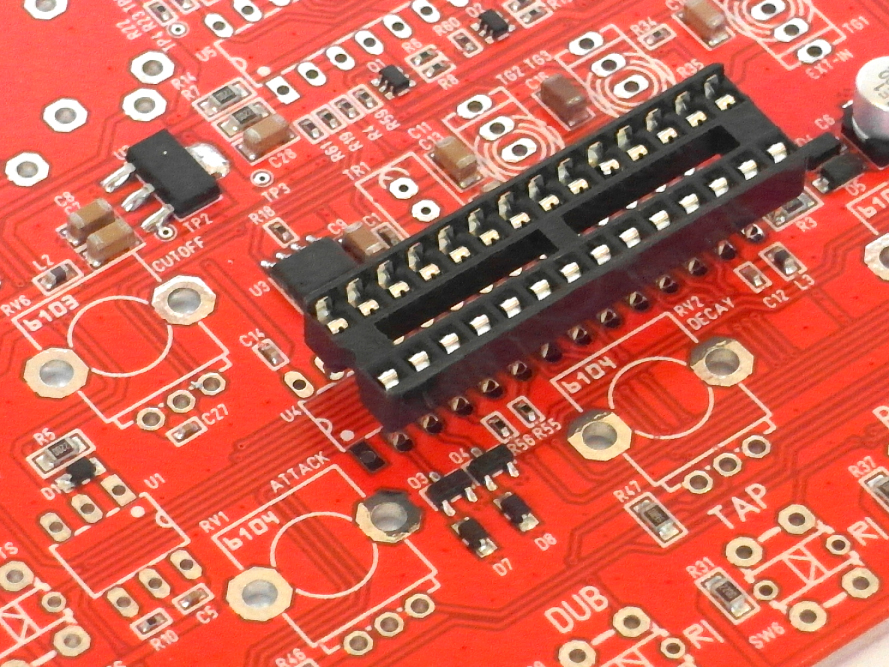
\includegraphics[scale=0.30]{assets/ic-socket.jpg}
        \caption{Inserting sockets}
    \end{center}
\end{figure}

The \textbf{IC sockets} have a \textbf{notch} on one side.
This marking must match the \textbf{footprint} drawn on the PCB \textbf{silk screen print}. The notch is represented by a semi-circle. The white point located next to it indicates the component pin number 1.

\begin{figure}[!ht]
    \begin{center}
        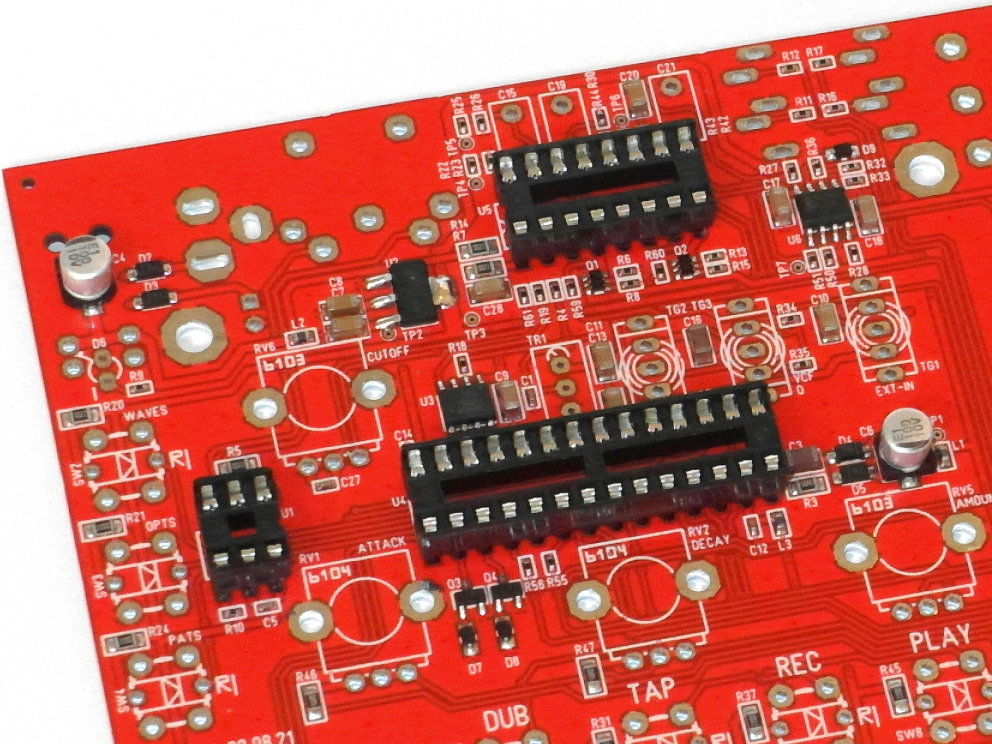
\includegraphics[scale=0.28]{assets/pcb-sockets.jpg}
        \caption{All sockets placed}
    \end{center}
\end{figure}
Take the necessary time to solder each socket pin and ensure there are \textbf{no solder bridges nor cold solder joints}. Once done, the board should ressemble the following picture.

\begin{figure}[!ht]
    \begin{center}
        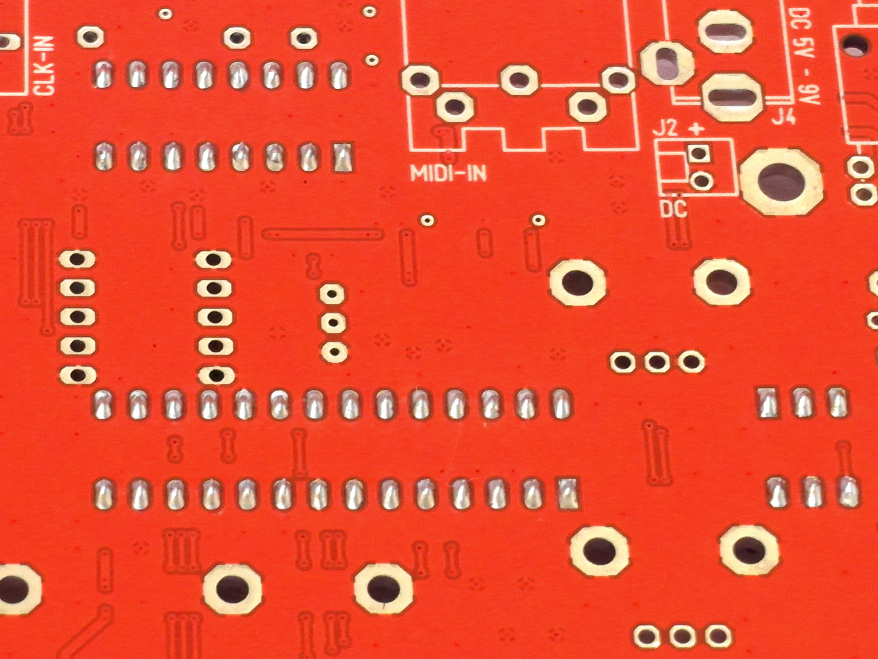
\includegraphics[scale=0.22]{assets/ic-solder.jpg}
        \caption{All sockets soldered}
    \end{center}
\end{figure}

\pagebreak
\subsubsection{Step 2: Film Capacitors}

The \textbf{film capacitors} are more \textbf{heat sensitive} than other parts. Do not heat the pins for a period longer than 5s.
These parts \textbf{are not polarized} and can be soldered in any orientation.

\begin{figure}[!ht]
    \begin{center}
        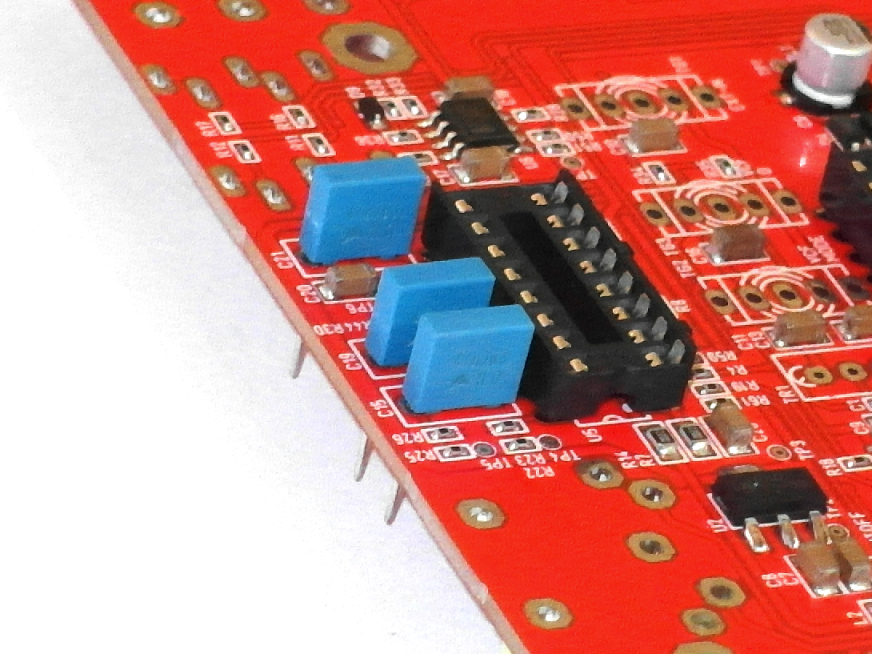
\includegraphics[scale=0.24]{assets/pcb-caps.jpg}
        \caption{Film capacitors}
    \end{center}
\end{figure}

After soldering, \textbf{trim off} the capacitors legs with a wire cutter, as shown on the picture.

\begin{figure}[!ht]
    \begin{center}
        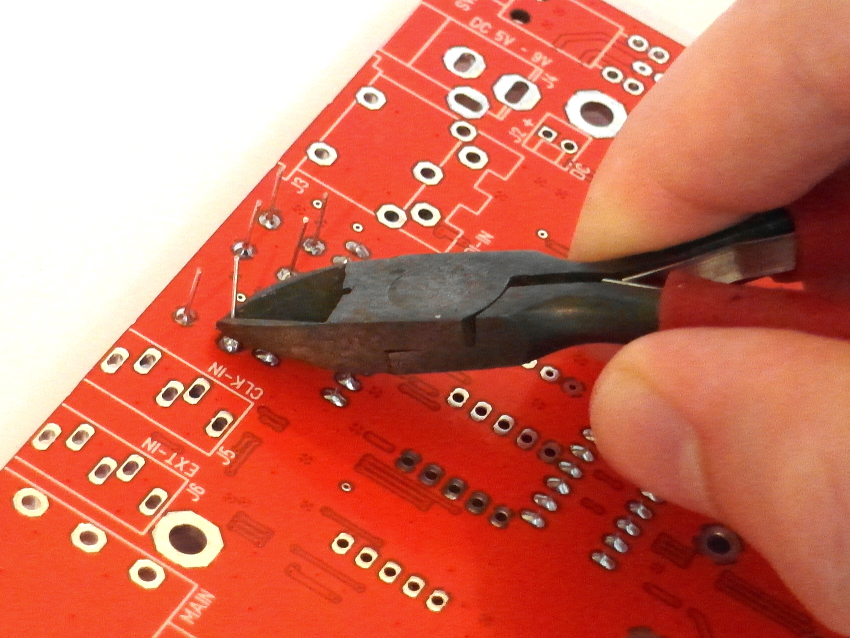
\includegraphics[scale=0.24]{assets/pcb-legs.jpg}
        \caption{Trimming legs}
    \end{center}
\end{figure}

\subsubsection{Step 3: Trimmer}

The \textbf{trimmer} is the blue part labeled \textbf{W103}. This component is not polarized and can be soldered in any orientation.

\begin{figure}[!ht]
    \begin{center}
        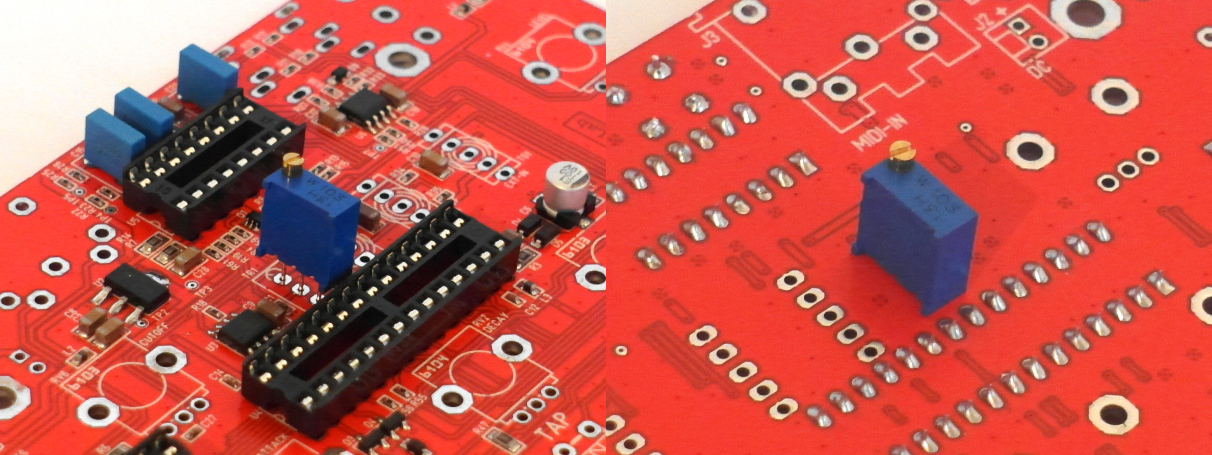
\includegraphics[scale=0.35]{assets/pcb-trimmer.jpg}
        \caption{Top or bottom configuration}
    \end{center}
\end{figure}

The trimmer can be installed at the \textbf{top or at the bottom} of the PCB. If you plan to give the \textbf{ZeKit} an enclosure, install the trimmer at the bottom and solder it later, at the connectors soldering step.

\subsubsection{Step 4: Tactile Switches}

While the \textbf{tactile switches} themself will work in all orientations, the built-in LEDs \textbf{have a polarity} which must be respected.

\begin{figure}[!ht]
    \begin{center}
        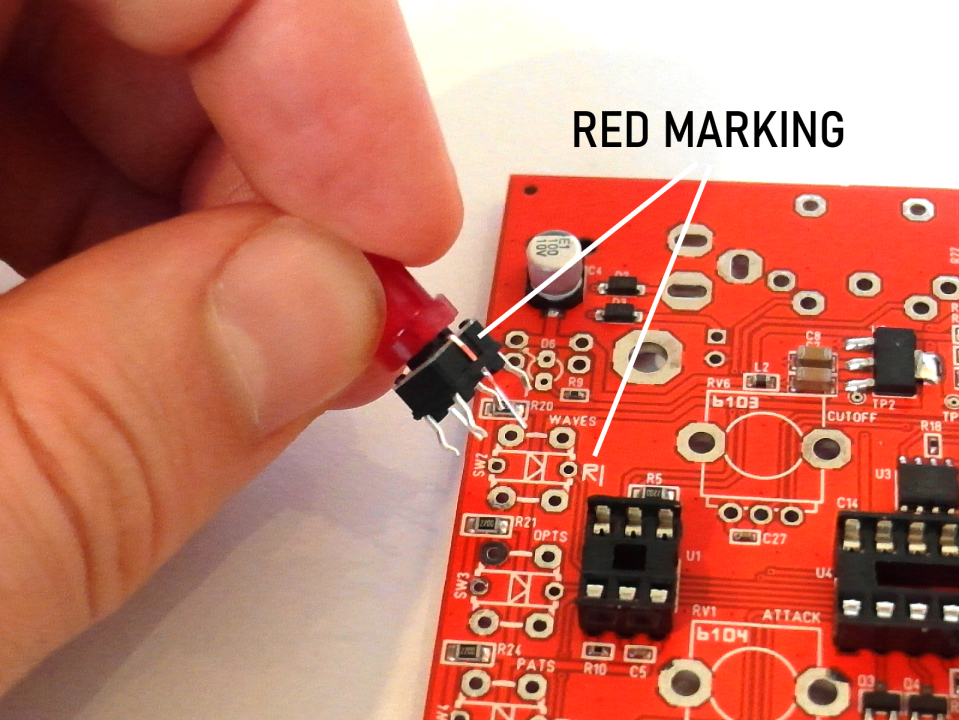
\includegraphics[scale=0.30]{assets/tact-marking.jpg}
        \caption{Mind the red leg!}
    \end{center}
\end{figure}

LED pins have different lengths. The longer pin also has a \textbf{red marking} and must be located on the \textbf{right side} of the switch.
Keep your attention \textbf{on soldering them straight.}

\subsubsection{Step 5: Toggle Switches}

The \textbf{toggle switches} are not polarized and can be soldered in any orientation.

\begin{figure}[!ht]
    \begin{center}
        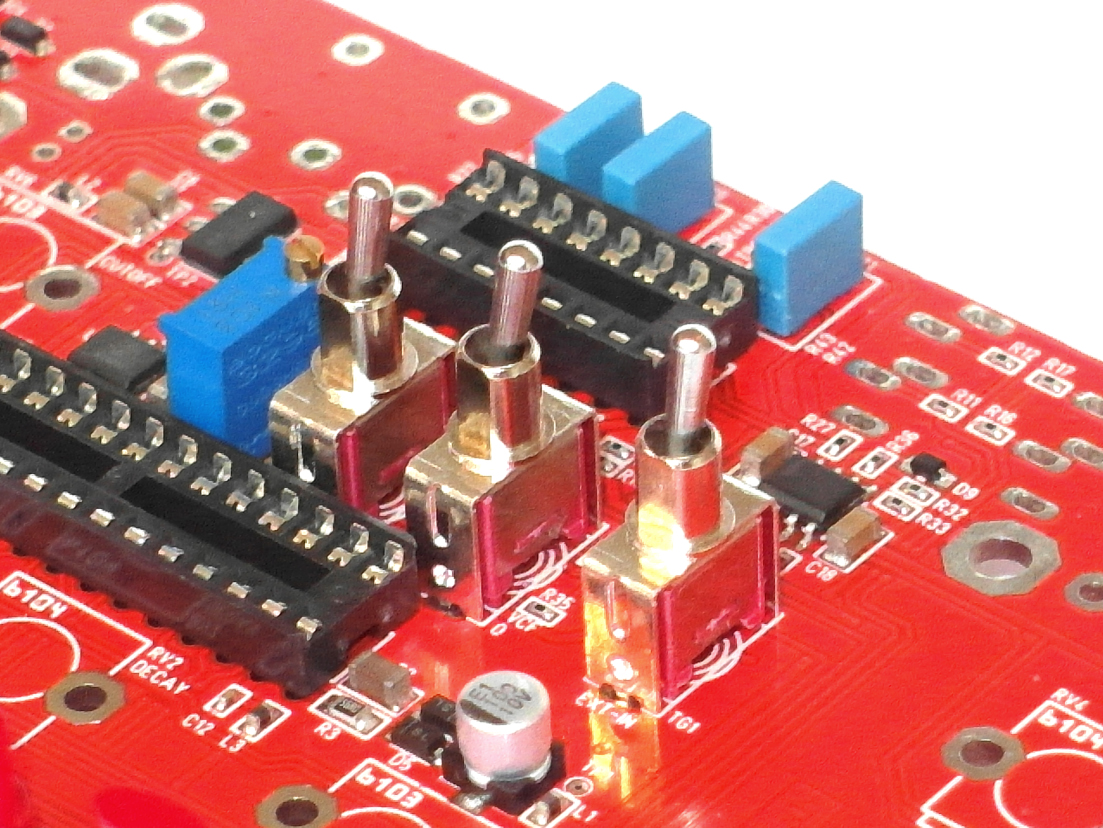
\includegraphics[scale=0.25]{assets/pcb-toggles.jpg}
        \caption{Mounted toggle switches}
    \end{center}
\end{figure}

\subsubsection{Step 6: Potentiometers}

There are \textbf{two potentiometer values} provided: \emph{10k and 100k Ohm.} \\
The \textbf{10k pots} are labeled \textbf{B103} at the bottom whereas the \textbf{100k} are labeled \textbf{B104}.

\begin{figure}[!ht]
    \begin{center}
        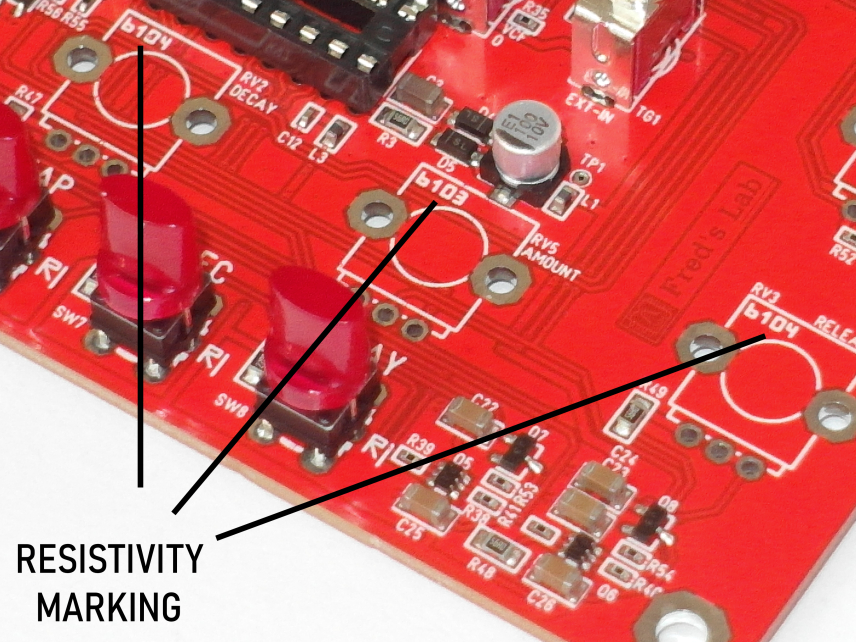
\includegraphics[scale=0.32]{assets/pots-marking.jpg}
        \caption{Pots resistivity marking}
    \end{center}
\end{figure}

To install the right pot at the right spot, \textbf{follow the markings} drawn on the PCB. \\
Also, keep your attention \textbf{on soldering the pots straight.}

\pagebreak

\subsubsection{Step 7: Power LED}

The \textbf{power LED} is a polarized component and must be installed \textbf{so its longer leg is the closest} to the \emph{SW2 tactile switch} (see picture).
The LED should be \textbf{mounted straight} on top at approximately \textbf{1cm} distance from the PCB surface.

\vspace{0.50cm}
\begin{figure}[!ht]
    \begin{center}
        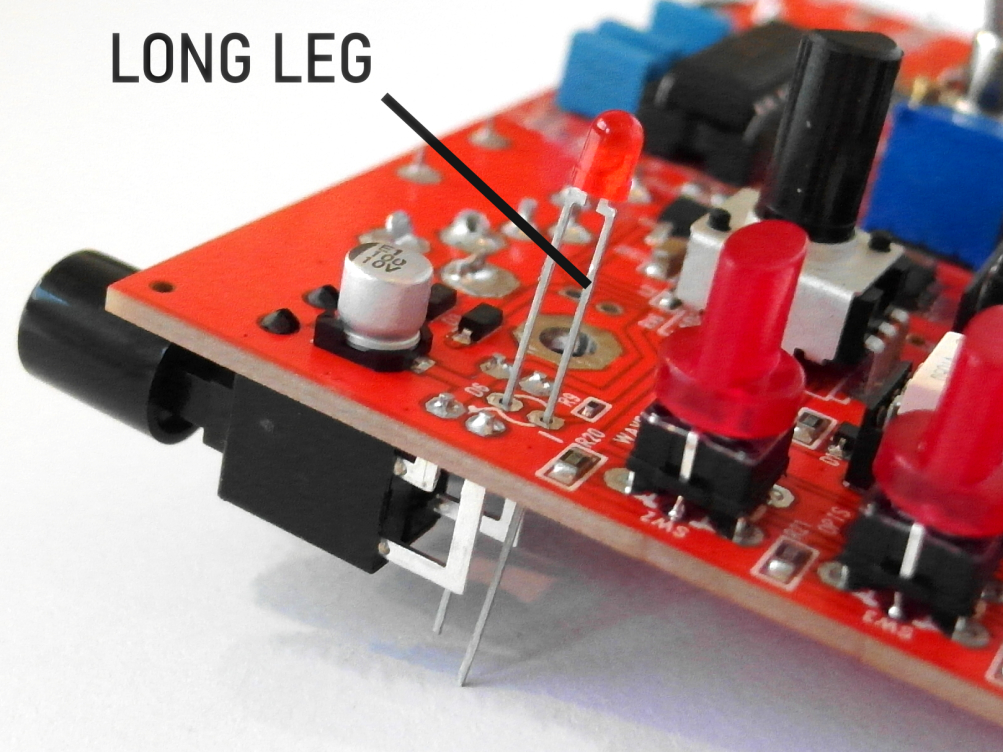
\includegraphics[scale=0.35]{assets/pcb-led.jpg}
        \caption{Power LED orientation}
    \end{center}
\end{figure}

Solder the long leg first and then adjust the LED height and alignment by reheating the solder joint.
Once you're satisfied with the LED position, solder the second leg and then trim them off with the cutter.

\subsubsection{Step 8: Connectors \& Power Switch}

\begin{figure}[!ht]
    \begin{center}
        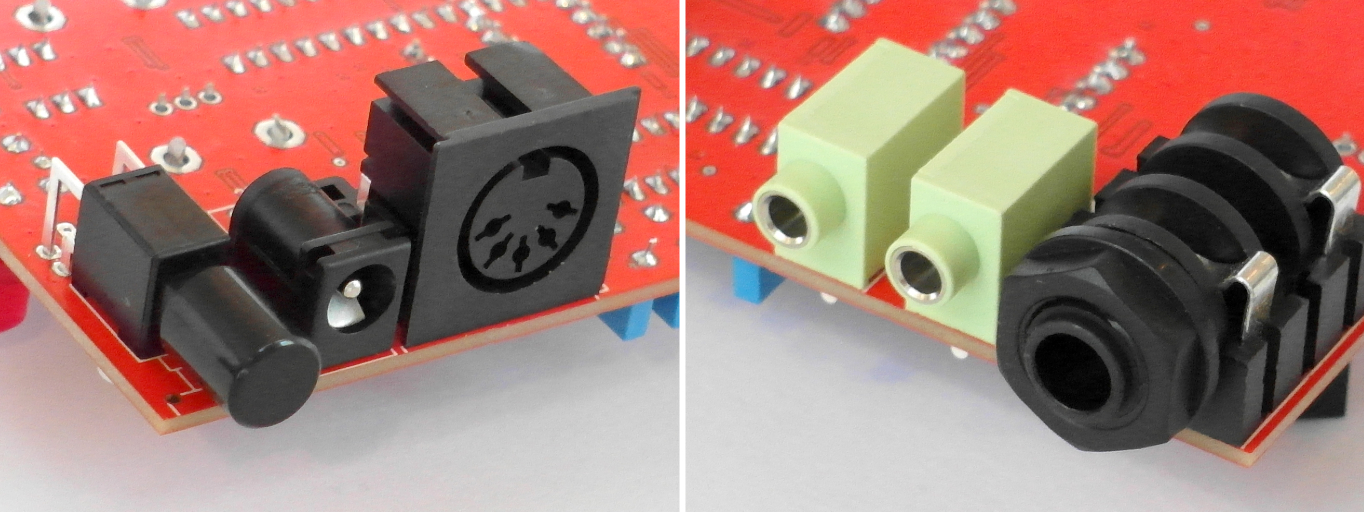
\includegraphics[scale=0.31]{assets/pcb-connectors.jpg}
        \caption{Bottom side connectors}
    \end{center}
\end{figure}

The \textbf{connectors \& power switch} are soldered last because they are located at the \textbf{bottom side} of the PCB.

If the \textbf{trimmer} wasn't installed at \emph{step 3,} you should solder it now.

\begin{figure}[!ht]
    \begin{center}
        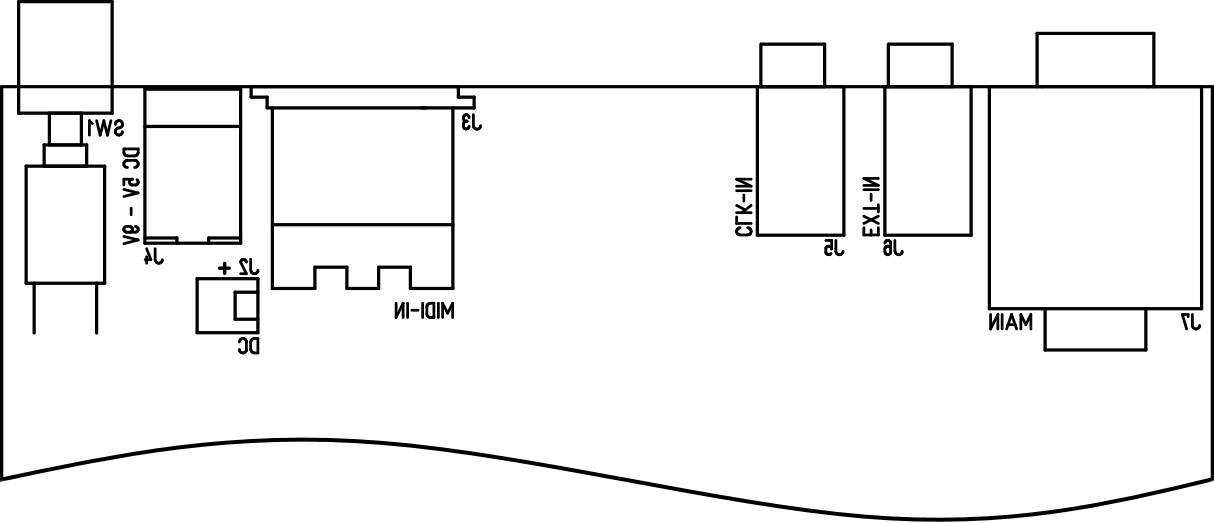
\includegraphics[scale=0.70]{assets/pcb-bot.png}
        \caption{Bottom placement diagram}
    \end{center}
\end{figure}

\subsubsection{Step 9: Inserting the ICs}

Now that the \textbf{ZeKit} is completely soldered, all ICs need to be inserted in their sockets, respecting the given orientation.

\vspace{0.50cm}
\begin{figure}[!ht]
    \begin{center}
        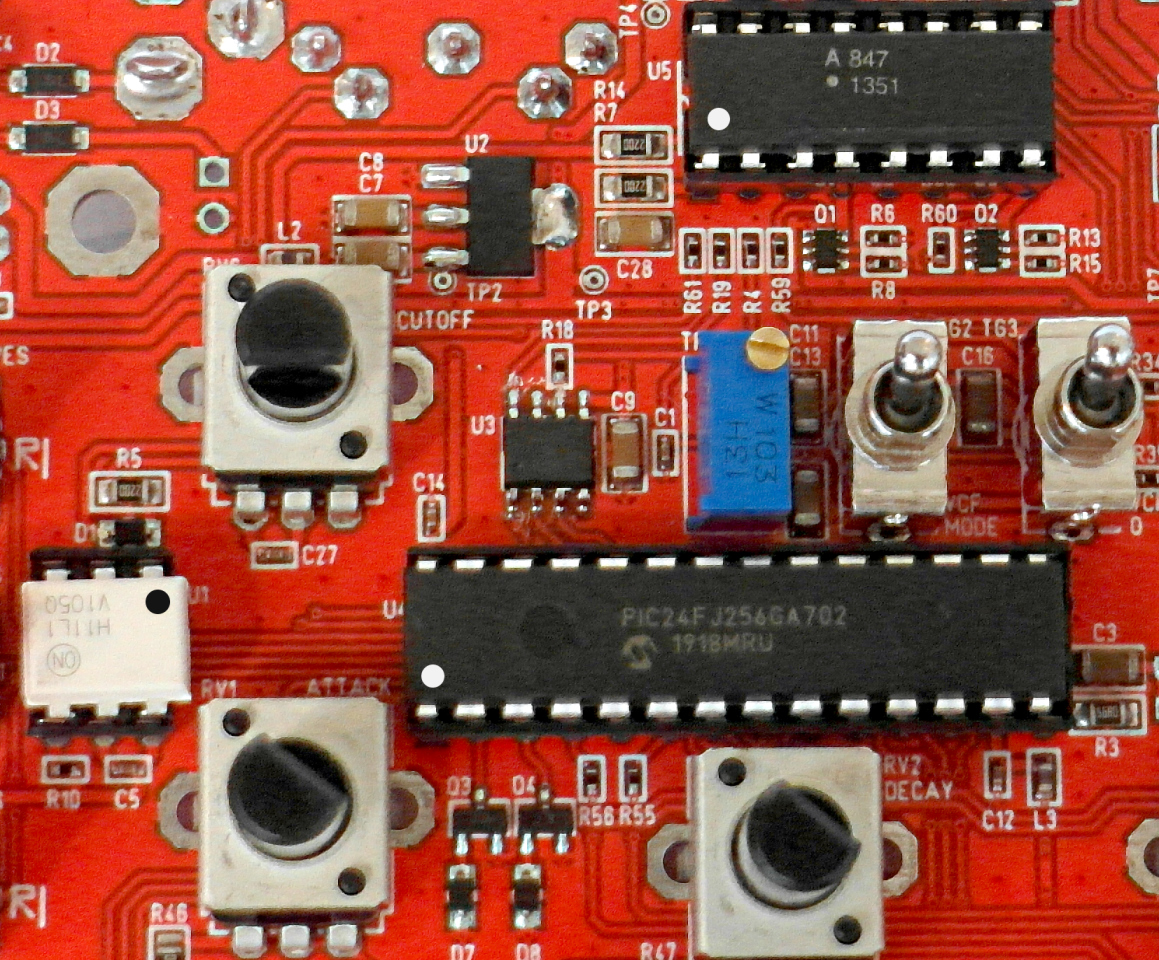
\includegraphics[scale=0.25]{assets/ic-orientation.jpg}
        \caption{Correct ICs orientation}
    \end{center}
\end{figure}

There are 3 different ICs:
\begin{itemize}
    \item \textbf{H11L1} (*) - "MIDI" optocoupler
    \item \textbf{LTV847} - VCF / VCA optocoupler
    \item \textbf{PIC24FJ256GA702} - 16bit microcontroller
\end{itemize}

(*) H11L1 can be shipped in black or white DIP (dual in-line package).

Before positioning the ICs, it is recommended to \textbf{carefully bend} their legs, so they are orientated more \textbf{parallel.} It will be easier to insert them in the sockets that way.

\vspace{0.25cm}
\begin{figure}[!ht]
    \begin{center}
        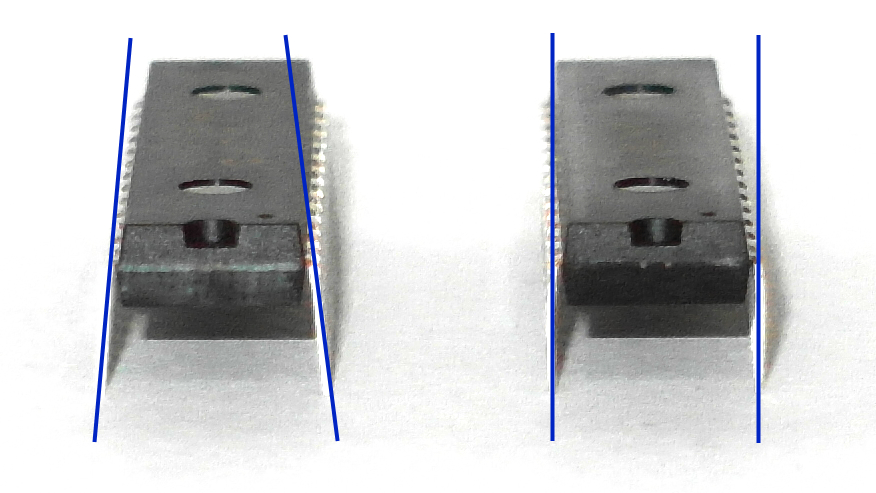
\includegraphics[scale=0.20]{assets/ic-bending.jpg}
        \caption{ICs parallel legs}
    \end{center}
\end{figure}

Verify the \textbf{ICs alignment} with their socket, make sure \textbf{no leg is pointing out}, and firmly press the ICs into their sockets.
\vspace{0.25cm}
\begin{figure}[!ht]
    \begin{center}
        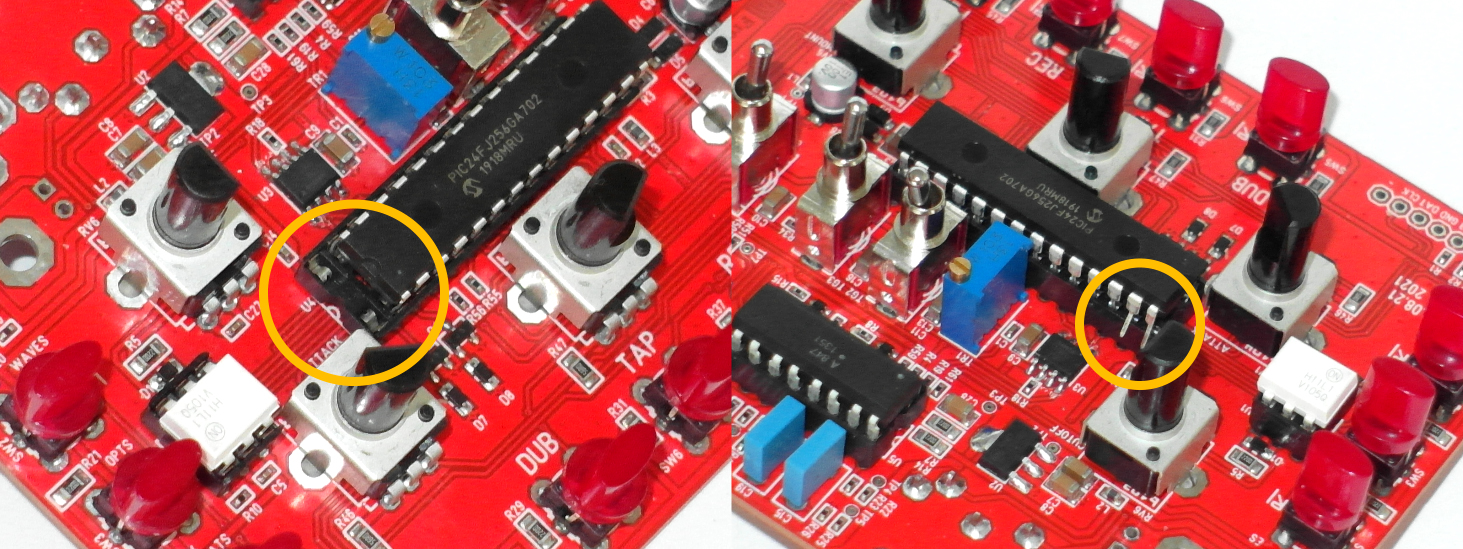
\includegraphics[scale=0.28]{assets/ic-incorrect.jpg}
        \caption{ICs mounted incorrectly}
    \end{center}
\end{figure}

\pagebreak
\section{Finishing the Kit}

\subsection{First Power Up}
\Large
\emph{Exciting moment ahead!}
\normalsize

Before powering up the \textbf{ZeKit} for the first time, \textbf{a last visual control} of the soldering job and a full check of the ICs orientation won't hurt.
For this, refer to the \textbf{component placement diagram.}

If this is your first build, try powering it up using \textbf{a lab power supply} or at least an adapter with some form of \textbf{current limiting.}
You don't want all your hard work going up in smoke!

Once turned on, the \textbf{power LED} should light up and \textbf{all tact switches} should blink when pushed. The \textbf{linear regulator} \emph{U2} must stay cool.
If you press the \textbf{play} switch \emph{SW8}, its function should latch, and the \textbf{tap} switch \emph{SW6} should blink regularly, indicating that the MCU is \textbf{correctly running the firmware.}

\vspace{0.5cm}
\textbf{Congratulations!}

Now, you can attach your \textbf{ZeKit} to a \emph{speaker system}, a \emph{MIDI controller} and \textbf{have a lot of fun} discovering your new instrument!

\begin{figure}[!ht]
    \begin{center}
        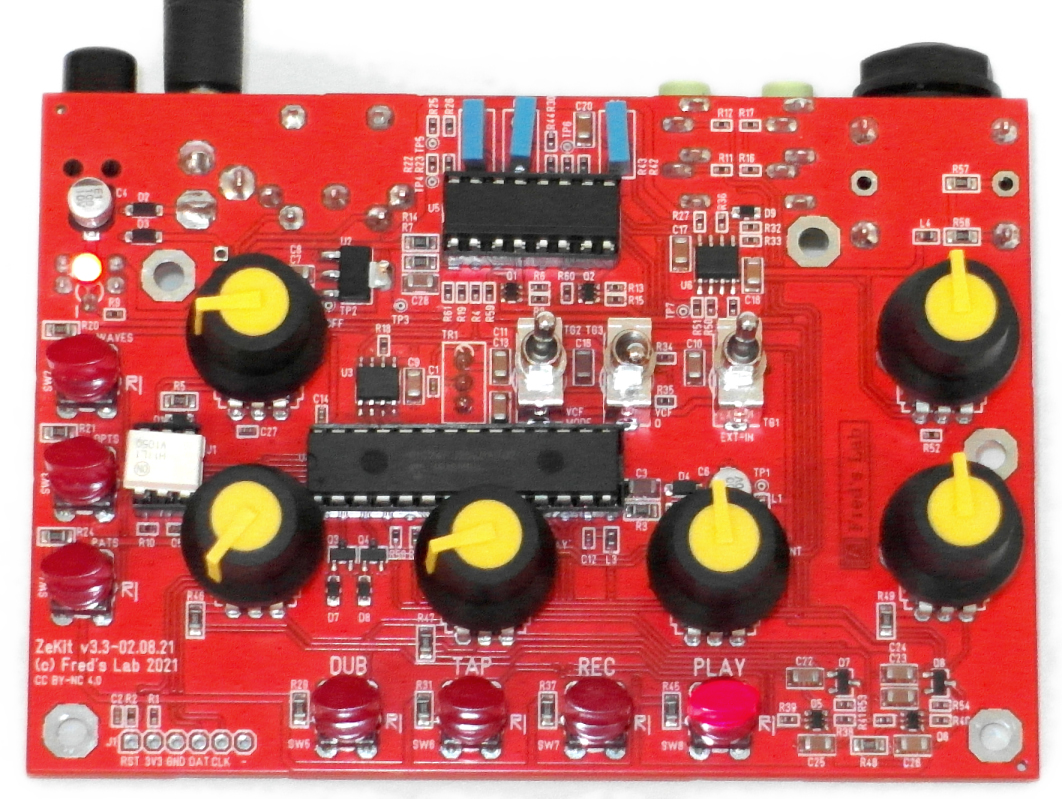
\includegraphics[scale=0.28]{assets/zekit-happy.jpg}
        \caption{An happy ZeKit!}
    \end{center}
\end{figure}

\vspace{0.5cm}
\textbf{IMPORTANT}

\begin{tcolorbox}
    \textcolor{red}{
        If what described isn't what you're getting... \textbf{immediately switch the power off} and read the \emph{Identifying Common Issues} section of this manual.
    }
\end{tcolorbox}

\pagebreak
\subsection{VCF Calibration}

\Large
\emph{Let's tweak this VCF!}
\normalsize

The \textbf{ZeKit} sound generation relies partly on \textbf{analog electronics} with their intrinsic manufacturing tolerances. Therefore, the filter will need some manual calibration.

The goal is to set the \textbf{VCF Cutoff Range} so the filter \emph{opens and closes} completely.

\begin{figure}[!ht]
    \begin{center}
        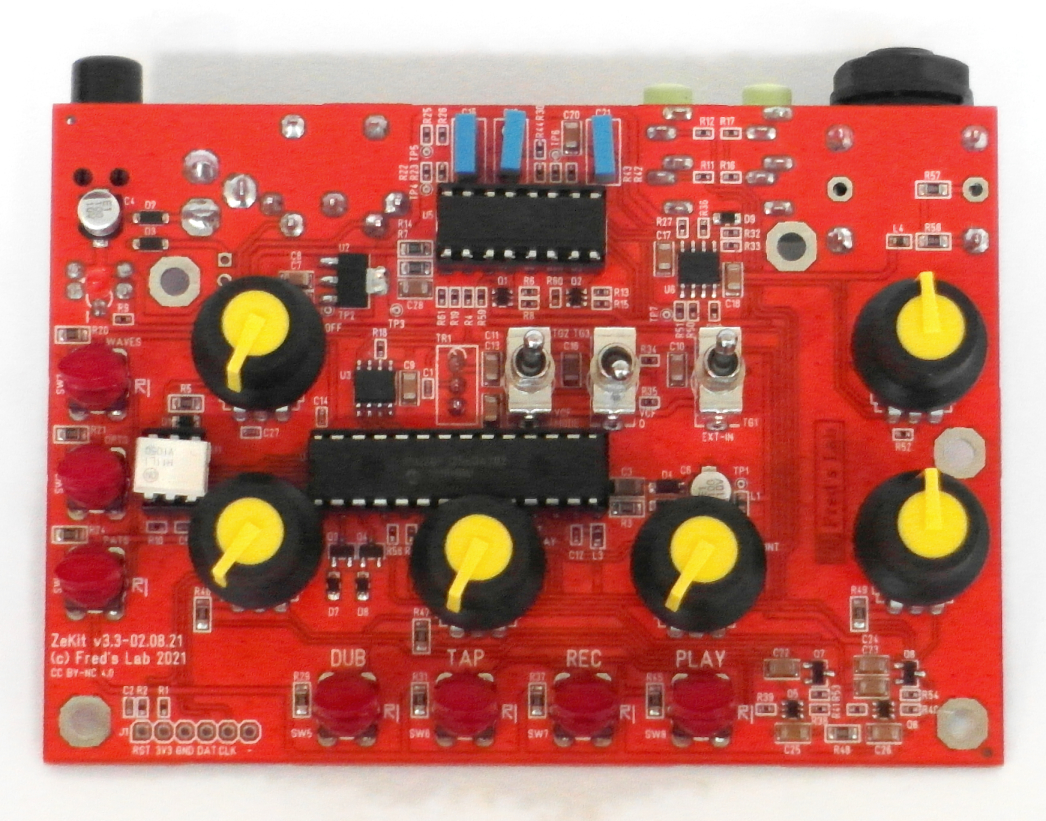
\includegraphics[scale=0.30]{assets/zekit-calibrate.jpg}
        \caption{Calibrating configuration}
    \end{center}
\end{figure}

To begin the calibration procedure, set the:
\begin{itemize}
    \item \textbf{Cutoff} pot \emph{RV6} to minimum
    \item \textbf{Attack} pot \emph{RV1} to minimum
    \item \textbf{Decay} pot \emph{RV2} to minimum
    \item \textbf{Accent} pot \emph{RV5} to minimum
    \item \textbf{Release} pot \emph{RV3} to center
    \item \textbf{Level} pot \emph{RV4} to center
    \item \textbf{VCF Mode} switch \emph{TG2} to top
    \item \textbf{VCF Q} switch \emph{TG3} to bottom
    \item \textbf{EXT IN} switch \emph{TG1} to top
\end{itemize}

\vspace{0.25cm}
Play some \textbf{very low notes} such as G1 (49Hz) or C1 (32Hz) using a \emph{MIDI keyboard} and \textbf{adjust the trimmer} \emph{TR1 screw} with a screw driver \textbf{until these notes are dampened.}

Finally, check the overall \emph{cutoff range} by sweeping the \textbf{Cutoff} pot \emph{RV6} and ensure that the filter \textbf{is opened completely} when the \textbf{cutoff} is at maximum. Adjust the trimmer \emph{TR1} accordingly.

\pagebreak
\subsection{What's Next?}

\textbf{ZeKit} has been designed to be more than a \emph{quickly assembled and affordable synth kit.}

The design material is provided under \textbf{Creative Commons (Schematics / PCB) and GNU GPL (Firmware) licenses} that allows you \textbf{to modify, extend and build upon} this project,
as long as it \textbf{isn't for commercial purposes} (or contact us).

\textbf{So let your imagination free,} here are areas to explore:

\begin{itemize}
    \item \textbf{Software modification} \\
          Firmware code is on GitHub
    \item \textbf{Hardware modding} \\
          Various test points are provided
    \item \textbf{Front panel design} \\
          Templates are on GitHub
    \item \textbf{Completely new housings}
    \item \textbf{Derivative work}
\end{itemize}

\subsection{Identifying Common Issues}

Here is a list of \textbf{the common troubles} you may be facing with:

\begin{itemize}
    \item Missing solder joints
    \item Cold solder joints - see picture
    \item Solder bridges - see picture
    \item Wrong component polarity
    \item Bad IC insertion
    \item Dead IC (overheated or shorted)
\end{itemize}

\vspace{0.50cm}

\begin{figure}[!ht]
    \begin{center}
        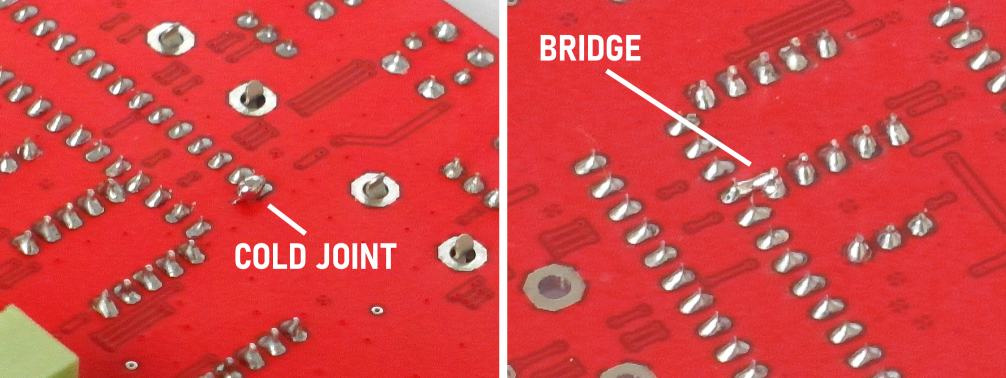
\includegraphics[scale=0.42]{assets/solder-issues.jpg}
        \caption{Soldering issues}
    \end{center}
\end{figure}

If you cannot figure out your build problems, please \textbf{write us an email} (with pictures) or \emph{kindly ask other users} who successfully assembled their \textbf{ZeKit}.

\pagebreak

% ------------------------------------------------------------------------------------------
\section{Functional Description}

\subsection{Power Supply}

The \textbf{ZeKit} needs energy delivered by the power supply. This block provides 3 voltages:
\begin{itemize}
    \item UNREG (what comes as input voltage)
    \item +3.3V using a \textbf{linear regulator}
    \item -2.0V using a \textbf{charge pump}
\end{itemize}

\subsubsection{Linear Regulator}

\vspace{-0.25cm}
\begin{center}
    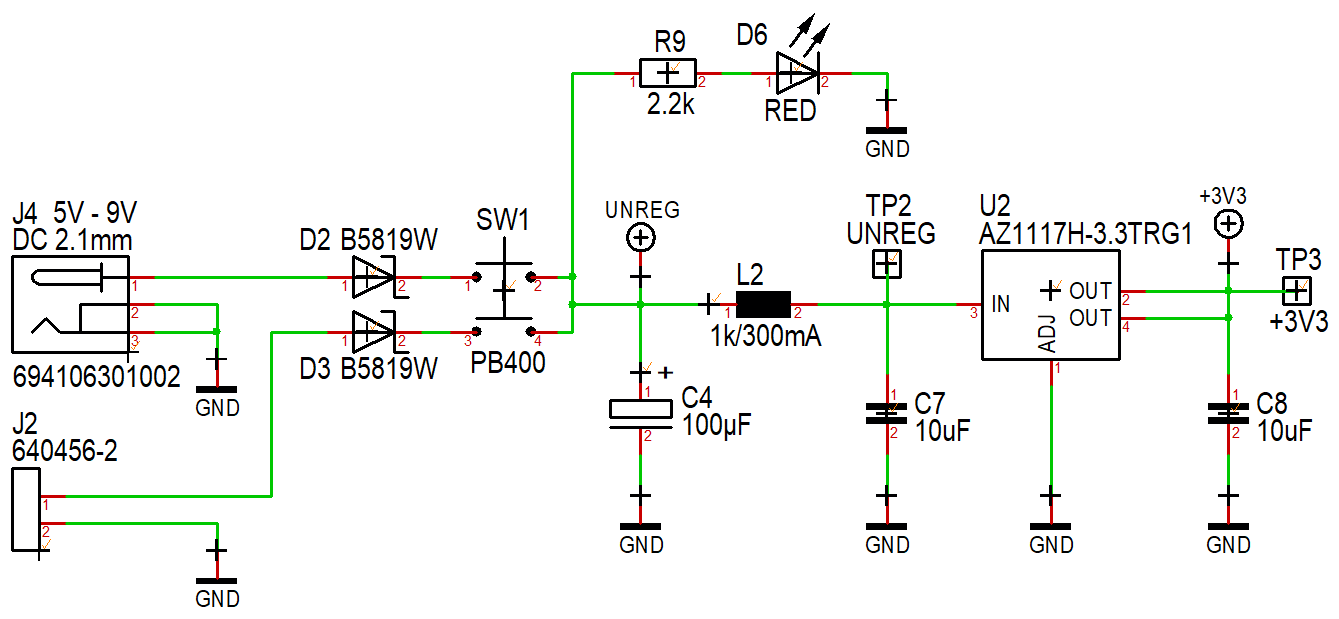
\includegraphics[scale=0.42]{assets/schema-power.png}
\end{center}

\emph{SW1} is the \textbf{power switch.} The diodes \emph{D2} \& \emph{D3} ensure a \textbf{correct voltage polarity,} by letting the current flows only in the right direction. The diodes also select which source - power adapter or battery - powers the \textbf{ZeKit}.

\emph{C4}, \emph{L2} \& \emph{C7} filter the input voltage, \textbf{reducing supply noise.} \emph{U2} regulates down the input, assuring a stable +3.3V in all circumstances. \emph{C8} secures \emph{U2} against possible oscillation of its output voltage.

\subsubsection{Charge Pump}

\begin{center}
    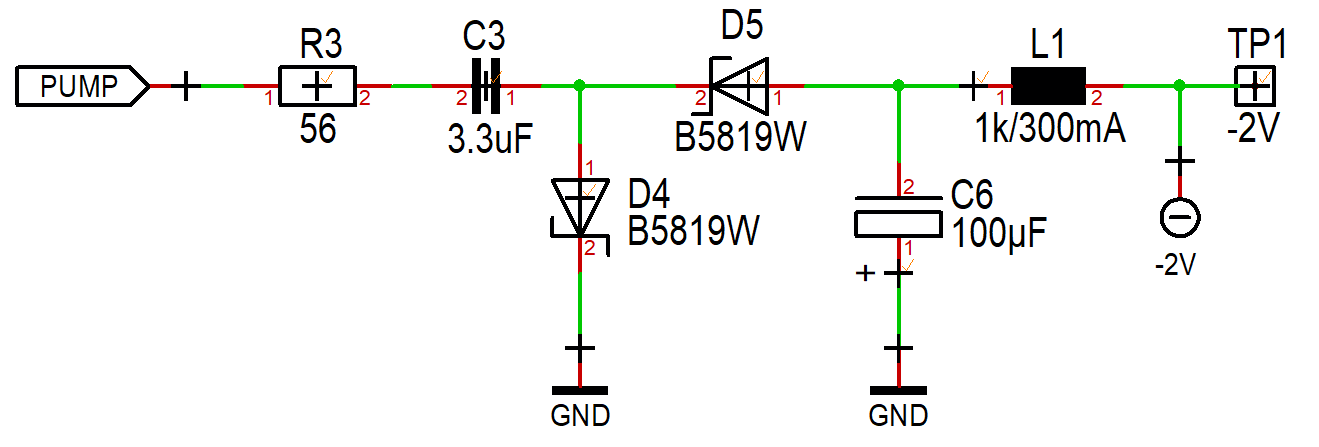
\includegraphics[scale=0.3]{assets/schema-pump.png}
\end{center}

The \emph{PUMP} signal is generated by the MCU and alternates between GND and +3.3V at a high frequency. When \emph{PUMP} is at +3.3V, \emph{C3} is charged via \emph{R3} and \emph{D4}, while \emph{D5} is non-conductive. When \emph{PUMP} is at GND, \emph{D4} is blocking and the charge of \emph{C3} is dumped through \emph{R3}, literally pumping charges from \emph{C6} via the now conducting \emph{D5}.

The inductor \emph{L1} filters the charge pump output voltage for better noise immunity.

Ideally, the output voltage at \emph{TP1} would be -3.3V, but because of the losses inside the diodes, it will be around -2V, which is sufficient for proper operation.

\subsection{PIC Microcontroller}

\begin{center}
    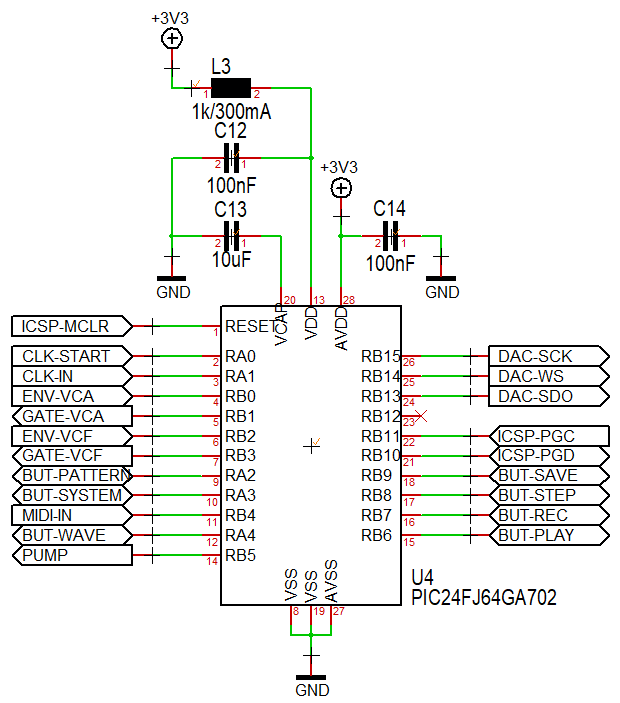
\includegraphics[scale=0.50]{assets/schema-mcu.png}
\end{center}

The \textbf{microcontroller} (MCU) \emph{U4} is the brain of the \textbf{ZeKit}. It processes all signals from the switches and the inputs and generates the audio waveforms as well as control signals for the analog circuitry. This is done by running a firmware that is stored in the internal flash of the chip.

The capacitors \emph{C12}, \emph{C13} and \emph{C14} are used together with the inductor \emph{L3} to improve the stability of the power supply and reduce noise propagation.

\subsection{DAC}

\begin{center}
    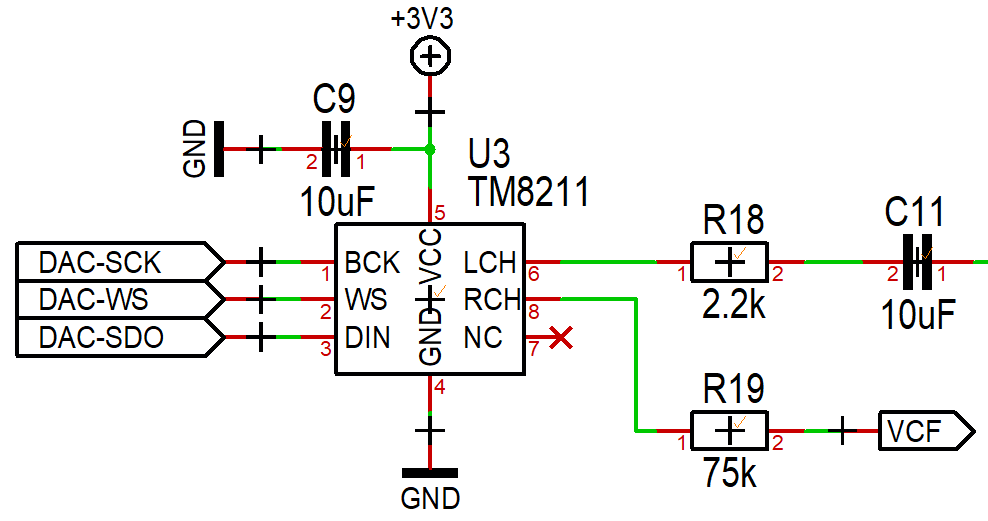
\includegraphics[scale=0.30]{assets/schema-dac.png}
\end{center}

The \textbf{digital-to-analog converter} (DAC) \emph{U3} is connected to the MCU via a standard signal bus, called \emph{I2S.} It converts the generated digital waveforms into a signal in the analog domain. Capacitor \emph{C11} removes the DC offset of the signal, resistor \emph{R18} \& \emph{R19} condition the levels to suit the VCF block inputs.

This DAC chip provides two independent output channels which are used as oscillators output and filter cutoff control.

\subsection{VCF}

\begin{center}
    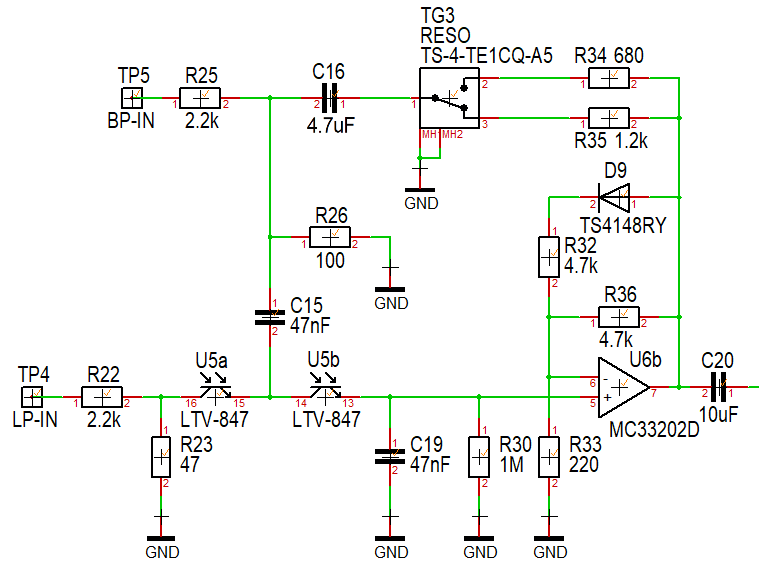
\includegraphics[scale=0.70]{assets/schema-vcf.png}
\end{center}
\vspace{0.25cm}

The \textbf{VCF} (voltage controlled filter) is a \textbf{2nd order design} with a 12dB/octave slope. The first stage consists of the optocouplers \emph{U5a \& U5b} and the capacitor \emph{C15}, the second stage of the optocoupler \emph{U5b} and the capacitor \emph{C19}. Here, the optocouplers play the role of the resistive elements to control the cutoff frequency.

The input signal \emph{VCF-IN} is fed in either to the first stage or the filter feedback path, depending whether low-pass or band-pass configuration is selected by the toggle switch \emph{TG2}. The resonance is determined by the feedback loop and can be chosen between two amounts via toggle switch \emph{TG3}.

The operational amplifier \emph{U6b} provides the necessary gain and low impedance to drive the next stage and the feedback loop. It uses the diode \emph{D9} to tame the amplitude at higher levels and produce a nice-sounding distortion.

\pagebreak
\subsection{VCA}
\vspace{0.25cm}
\begin{center}
    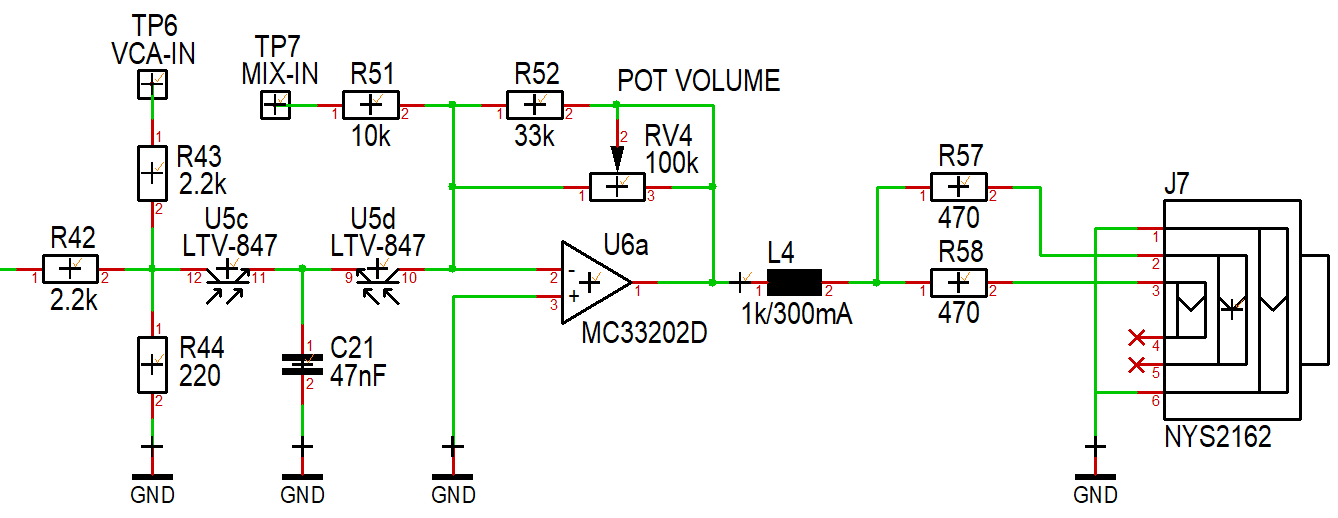
\includegraphics[scale=0.40]{assets/schema-vca.png}
\end{center}

The \textbf{VCA} (voltage controlled amplifier) uses the optocoupler \emph{U5c/U5d} to gain-control the operational amplifier \emph{U6a}. The input signal \emph{VCA-IN} is decoupled by capacitor \emph{C20} and then divided down by resistors \emph{R42} and \emph{R44} to an appropriate level for the optocoupler.

To set the output level, the \textbf{Volume} potentiometer is part of the feedback path of the opamp. Resistor \emph{52} in parallel to the pot provides a nicer control curve for the volume setting.

The output is RF filtered by inductor \emph{L4}, followed by protection resistors \emph{R57} and \emph{R58} and then routed to the output jack \emph{J7}.

\subsection{Envelopes}

\subsubsection{VCF Envelope}

\begin{center}
    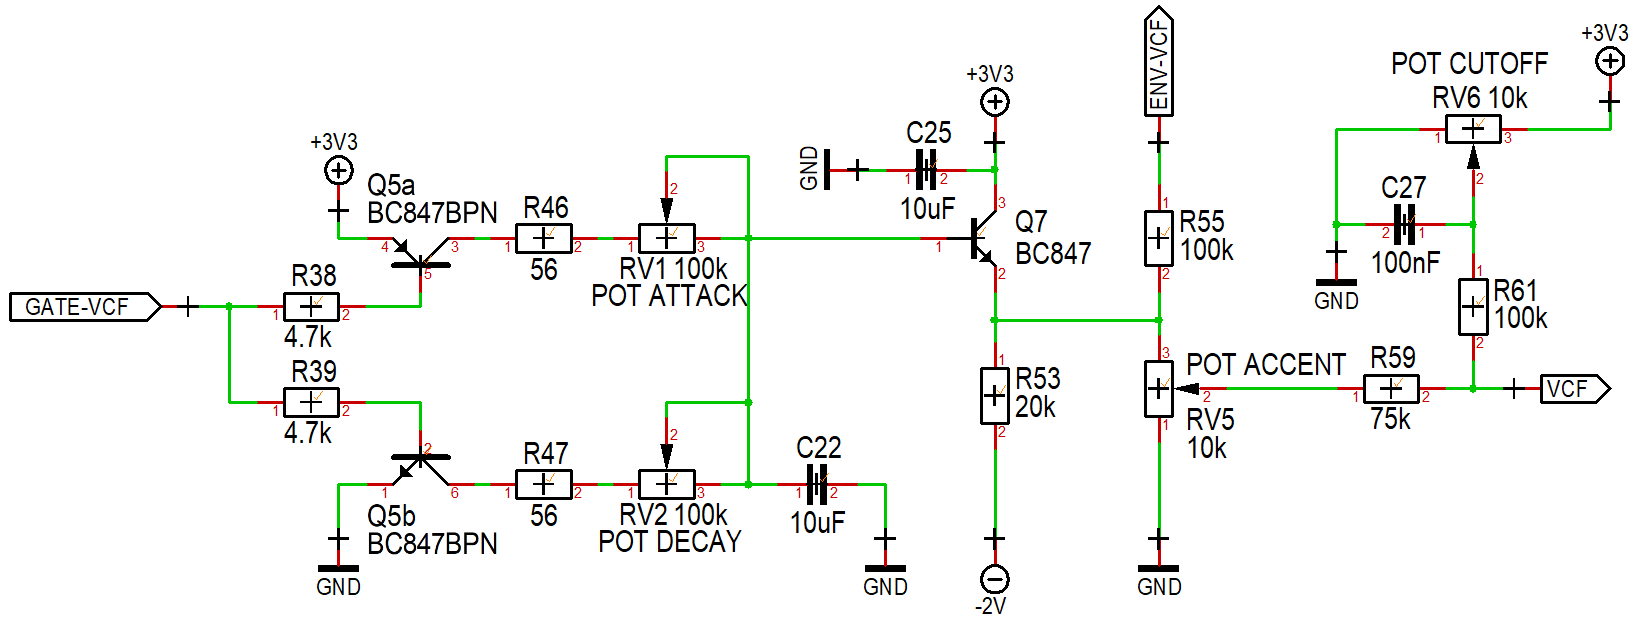
\includegraphics[scale=0.35]{assets/schema-ar-vcf.png}
\end{center}

The \textbf{filter envelope} is generated by either charging capacitor \emph{C22} to +3.3V or discharging it to GND.
To trigger the envelope, the MCU sets the \emph{GATE-VCF} signal to GND. The transistor \emph{Q5a} then conducts and \emph{C22} is charged via the resistor \emph{R46} and the \textbf{Attack} potentiometer.

To release the envelope, the MCU sets the \emph{GATE-VCF} signal to +3.3V. \emph{Q5a} then cuts off and \emph{Q5b} starts to conduct, resulting in \emph{C22} being discharged via \emph{R47} and the \textbf{Release} potentiometer.

The transistor \emph{Q7} acts as a buffer to decouple the envelope and prevent \emph{C22} to loose its charge. The \emph{ENV-VCF} signal is routed back to the MCU so it can detect when the \emph{attack phase} is finished. Finally, the envelope amount is controlled by the \textbf{Accent} potentiometer and added to the constant level set by the \textbf{Cutoff} potentiometer.

\subsubsection{VCA Envelope}

\begin{center}
    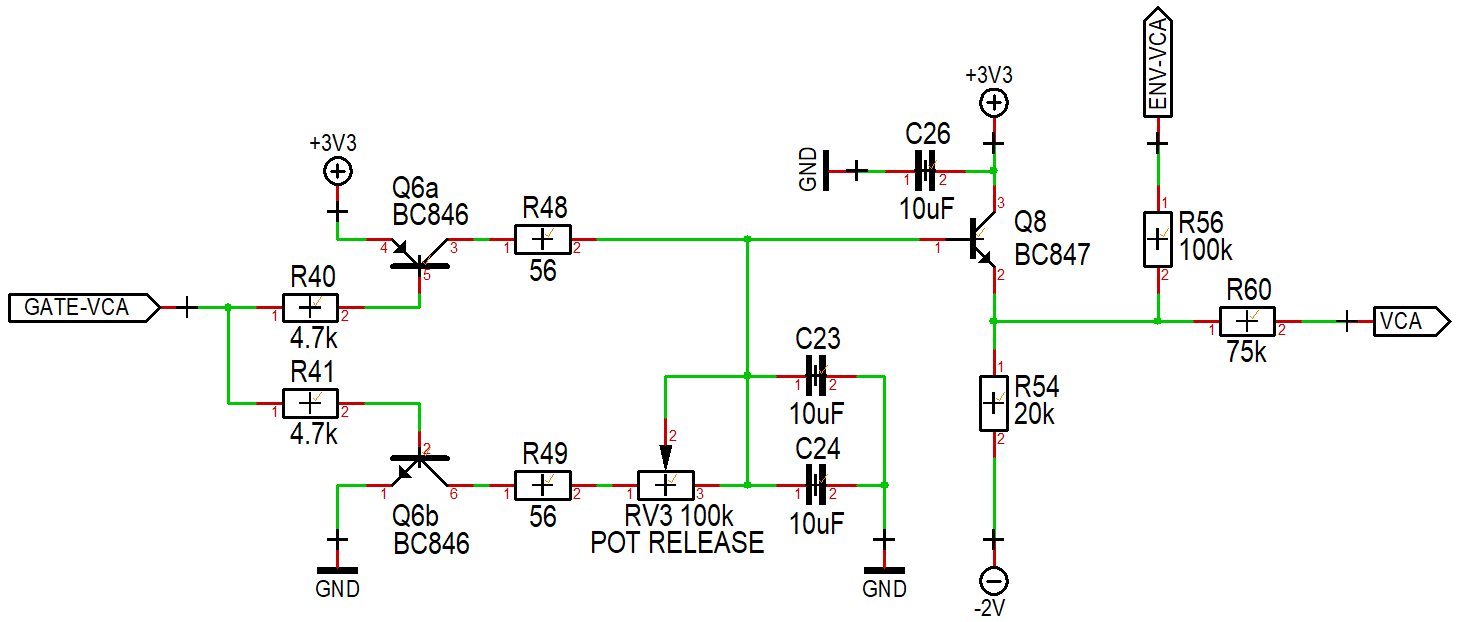
\includegraphics[scale=0.38]{assets/schema-ar-vca.png}
\end{center}

The \textbf{amplifier envelope} is a simplified version of the filter envelope. It works the same but lacks the \textbf{Attack} and \textbf{Amount} controls.

\subsection{Exponential Control Circuits}

\begin{center}
    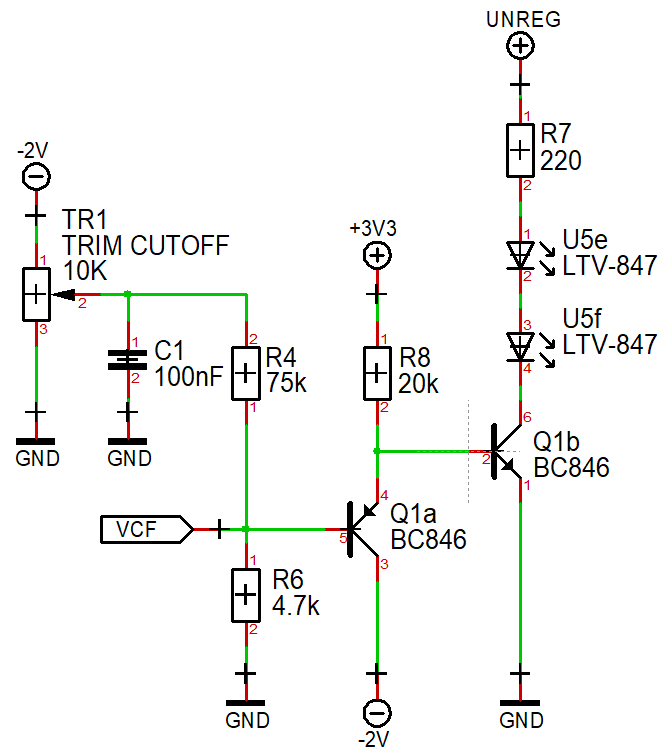
\includegraphics[scale=0.42]{assets/schema-expo-vcf.png}
    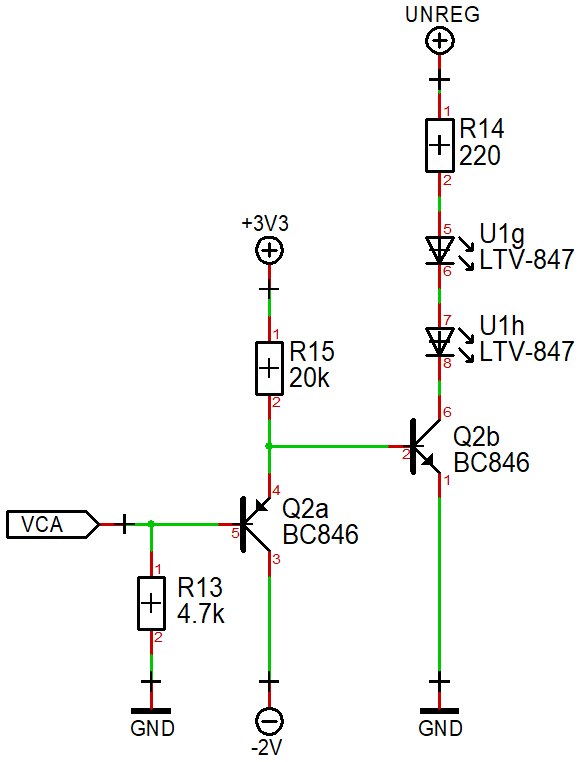
\includegraphics[scale=0.42]{assets/schema-expo-vca.png}
\end{center}

This \textbf{exponentiator circuit} converts the linear control voltage into \textbf{an exponential current} to drive the optocouplers LEDs.
The requirement for this is the \emph{nature of our human hearing} which recognizes pitches and volumes in an exponential way.

\pagebreak
The signal \emph{VCF} comes from the filter envelope and drives the buffer transistor \emph{Q1a}.

The trim potentiometer \emph{TR1} adds an offset to the input to calibrate the filter cutoff range. The emitter of \emph{Q1a} drives the base of transistor \emph{Q1b} which does the curve conversion.
It exploits the exponential relationship between the base-emitter voltage and the collector current of a transistor.
The collector current of \emph{Q1b} drives the LEDs inside the optocoupler \emph{U5}, controlling the filter cutoff.

The VCA uses a similar circuit that is driven by the \emph{VCA} signal coming from the amplifier envelope.

\subsection{MIDI Input}

\begin{center}
    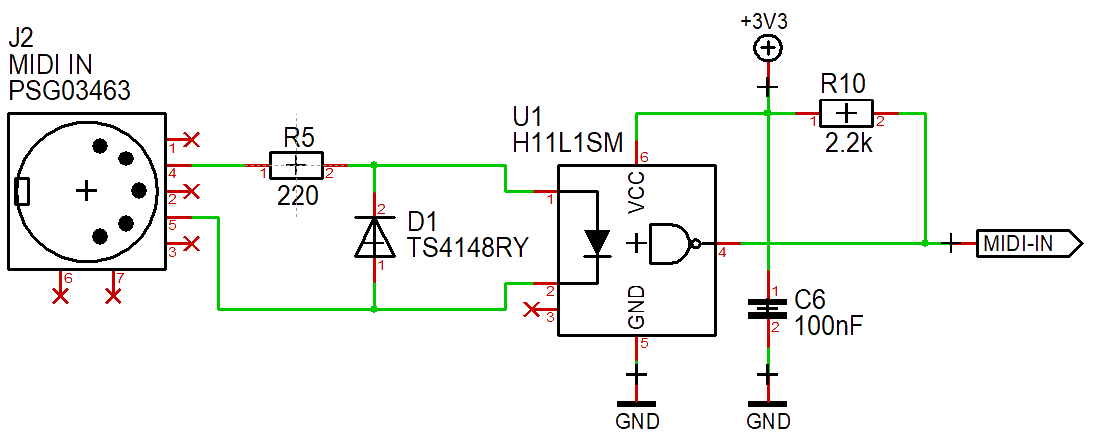
\includegraphics[scale=0.68]{assets/schema-midi.png}
\end{center}

The \textbf{MIDI input} is electrically isolated from the attached MIDI gear by using an optocoupler (this time in their intended usage) to prevent ground loops and the commonly associated audio noises.
This is required by the \emph{official MIDI specification.}

The external MIDI device drives the optocoupler \emph{U1} internal LED via the resistor \emph{R5}. When the LED is on, the phototransistor conducts and the \emph{MIDI-IN} signal is pulled to GND.
When the LED is off, the phototransistor cuts off and \emph{MIDI-IN} is set to +3.3V, by the pull-up resistor \emph{R10}.

The diode \emph{D1} clamps potential reverse spikes due to static electricity and prevents optocoupler LED being damaged.

\pagebreak
\subsection{Clock Input}

\begin{center}
    \includegraphics[scale=0.40]{assets/schema-clocks.png}
\end{center}

The \textbf{clock signal} is taken from the tip of the input jack \emph{J5}. Depending on the input voltage, the transistor \emph{Q4} is either conducting or not. Resistor \emph{R12} and diode \emph{D8} protect the transistor against over-voltage or wrong polarity at the input.

At the end, the signal \emph{CLK-IN} is routed to the microcontroller. The MCU uses an internal pull-up resistor to detect the high level when the transistor \emph{Q4} is off.

The \textbf{start signal} is taken from the ring of the input jack and processed in a similar fashion by driving the transistor \emph{Q3} to generate the \emph{CLK-START} signal for the MCU.

\subsection{Tactile Switches}

\vspace{0.50cm}
\begin{center}
    \includegraphics[scale=0.35]{assets/schema-switch.png}
\end{center}

The \textbf{illuminated tactile switches} are directly connected to the microcontroller.

To reduce the number of required signals, the MCU firmware uses a neat trick: \\
It alternates the MCU pin mode connected to the switch signal between input and open-drain (like a switch to ground) modes.

When the MCU pin is \textbf{configured as an input,} the button state can be read.
When the button is released, a high level is detected, because the pin is connected to +3.3V via the LED and the limiting resistor.
When the button is pressed, the pin is directly connected to GND and a low level is detected.

When the MCU pin is \textbf{configured as an output,} the switch LED can be switched on by driving the control signal to GND and switched off by letting the signal "floating" (or set to high-impedance).

% ------------------------------------------------------------------------------------------
\pagebreak
\section{Additional Resource}
You will find plenty of \textbf{additional resource} (graphic files, firmwares, sources, template, manuals...), at the following addresses:

\vspace{0.25cm}
\begin{itemize}
    \item \textbf{GitHub (source code, design files)} \\
          https://github.com/Marzac/zekit
          \vspace{0.25cm}
    \item \textbf{Fred's Lab Website} \\
          https://fredslab.net/en/zekit-module.php
\end{itemize}

\vspace{0.25cm}
Community created material, videos, sounds and links will be added as the project grows!

% ------------------------------------------------------------------------------------------

\section{Legal Notices}

\textbf{Fred's Lab} cannot be liable for erroneous information contained in this manual. Its contents may be updated without prior notice. We have put our best effort to ensure the information provided here is \textbf{useful and accurate.} \textbf{Fred's Lab} extends no liabilities in regard to this manual other than those required by the local laws.

\vspace{0.25cm}
\begin{center}
    \textbf{Frédéric Meslin Audiogeräte} \\
    Herwarthstraße, 20 \\
    53115 Bonn, Germany \\
    \url{info@fredslab.net} \\
    \url{http://fredslab.net} \\
\end{center}

\vspace{0.25cm}
\textbf{Support requests} \\
For support requests, you can reach us per e-mail at:
\begin{center}
    \url{support@fredslab.net}
\end{center}
or per post, using the company address.

For each support request, please include the \textbf{product model, serial number} and a \textbf{precise description} of the problem encountered with a maximum of details and supporting elements for a quick resolution.

\vspace{0.5cm}
\textbf{Copyright information}

This original manual, its content (including all graphics, pictures \& description) are the property of \textbf{Fred's Lab}. No part of this manual should be reproduced other than for private use and backup needs without a \emph{written permission} from \textbf{Fred's Lab}.

\pagebreak

% ------------------------------------------------------------------------------------------
\section{Schematics}
\textbf{Schematics} are provided under the Creative Commons \textbf{CC BY-NC licence}.\\\\
This license allows you to \textbf{remix, adapt, and build upon} this work non-commercially, provided that the derivative works acknowledge the contributions of the original author.
\vspace{0.25cm}
\begin{center}
    \includegraphics[scale=0.72,origin=c]{assets/schema-full.png}
\end{center}

\section{Bill Of Material}
\vspace{0.25cm}
\begin{center}
    \includegraphics[scale=0.72,origin=c]{assets/bom.png}
\end{center}

\end{document}
